%http://texblog.org/2011/09/09/10-ways-to-customize-tocloflot/

%Автоматически вписывать картинки в ширину страницы:
%\includegraphics[maxwidth=\linewidth]{foobar}

\documentclass[11pt,a4paper,notitlepage]{report}
\makeatletter
\newcommand*{\toccontents}{\@starttoc{toc}}
\makeatother
%\usepackage{pscyr}
\usepackage[utf8]{inputenc}
%\renewcommand{\rmdefault}{ftm}
\renewcommand{\rmdefault}{CMR}
\usepackage[russian]{babel}

\pagestyle{plain} % нумерация страниц вкл.

%\setmainfont{Имя шрифта}
%http://tex.stackexchange.com/questions/181183/combine-usepackagetimes-and-fontspec-setmainfont
%http://andreyolegovich.ru/PC/LaTeX.php#base
\usepackage{amsmath}
\usepackage{graphicx}
\usepackage{pdfpages}
\usepackage{comment}
\usepackage{textcomp}
\usepackage{wrapfig}
\usepackage{sectsty}
\usepackage{lipsum}
\usepackage{fancyhdr}
\usepackage{datetime}
%\allsectionsfont{\centering}
\chapterfont{\centering}
\usepackage[T2A]{fontenc}
\usepackage{lscape}
\usepackage{makecell}
\usepackage{multicol}
\usepackage{titlesec}
\usepackage{floatrow}
\usepackage{float}
\usepackage{caption}


\graphicspath{{img/}}

%*****************************************************
% Часто требуется, чтобы номер рисунка содержал в себе номер главы (вроде Рис. 1.1). Чтобы была сделана нумерация по главам, достаточно изменить счётчик рисунков в преамбуле документа вот так:
\renewcommand{\thefigure}{\thesection.\arabic{figure}}
%*****************************************************

%*****************************************************
%Если вас не устраивает вид подрисуночной подписи (например, вместо "Рис. 1:" необходимо "Рис. 1 --- "), используйте пакет caption. В частности, для установки тире в качестве разделителя, вставьте в преамбулу документа следующий код: 
\RequirePackage{caption}
\DeclareCaptionLabelSeparator{defffis}{ --- }
\captionsetup{justification=centering,labelsep=defffis}
%*****************************************************

%\usepackage[colorlinks=true,linkcolor=blue]{hyperref}

%*****************************************************
%Как сделать, чтобы уравнения нумеровались независимо по главам в LaTeX?
%В преамбуле
\makeatletter \@addtoreset{equation}{section} \makeatother 
\makeatletter \@addtoreset{figure}{section} \makeatother 
%*****************************************************

\addto\captionsrussian{
	\def\figurename{Рисунок}
}


\usepackage[hypcap]{caption}

%*****************************************************
% Начинать секции с новой страницы
%\usepackage{titlesec}
%\newcommand{\sectionbreak}{\clearpage}
%*****************************************************


%*****************************************************
%Чтобы в генерированном PDF работали гиперссылки, то надо подключить модуль hyperref (и если хотите их разрисовать, то модуль по работе с цветами xcolor):
\usepackage{xcolor}
\usepackage{hyperref}
% Цвета для гиперссылок
\definecolor{linkcolor}{HTML}{012b37} % цвет ссылок
\definecolor{urlcolor}{HTML}{012b37} % цвет гиперссылок
\hypersetup{pdfstartview=FitH,  linkcolor=linkcolor,urlcolor=urlcolor, colorlinks=true}
%*****************************************************

%***************************************************** 
%Для удаления номеров страниц из \listoffigures
\makeatletter
\newcommand{\emptypage}[1]{%
	\cleardoublepage
	\begingroup
	\let\ps@plain\ps@empty
	\pagestyle{empty}
	#1
	\cleardoublepage}
\makeatletter
%*****************************************************


\setcounter{secnumdepth}{3}
%\usepackage{enumitem}
\usepackage[shortlabels]{enumitem}
\setlist[enumerate]{leftmargin=*,align=left,label=\thesubsection.\arabic*.}
%\usepackage{enumerate}

\usepackage{lastpage} 

\usepackage{longtable}




%\renewcommand{\rmdefault}{ftm}
\renewcommand{\rmdefault}{cmr}
\renewcommand{\thesection}{\arabic{section}}
%\usepackage{enumitem}
%%% Страница
%\usepackage{extsizes} % Возможность сделать 14-й шрифт
\usepackage{geometry} % Простой способ задавать поля
\geometry{top=15mm}
\geometry{bottom=10mm}
\geometry{left=10mm}
\geometry{right=10mm}

%*****************************************************
%Here is how you can increase the space between the number and the caption in your \listoffigures. Add the following two lines before your \begin{document}:
\usepackage{tocloft}
\setlength{\cftfignumwidth}{3em}
%With the tocloft-package you can control the design of table of contents, figures and tables.
%*****************************************************


\usepackage{svn}

\pagestyle{fancy}
%\fancyfoot[]{вер. 1.05}
\fancyfoot[]{Страница \thepage \; из \pageref{LastPage}}
\renewcommand{\headrulewidth}{0pt}
\renewcommand{\footrulewidth}{0pt}
\setlength\headheight{80.0pt}
\addtolength{\textheight}{-80.0pt}
\chead{
\includegraphics[width=\textwidth]{img/log1o.png}}
\cfoot{
\includegraphics[width=\textwidth]{img/foot.png}}





%*****************************************************
%Номера страниц, включающие номер главы
\usepackage[auto]{chappg} %%% this is to set the page numbers as Chapter-Page.
%*****************************************************



\newdate{date}{28}{01}{2016}
\date{\displaydate{date}}
%Increase the value of tocdepth and secnumdepth. The tocdepth value determines to which level the sectioning commands are printed in the ToC (they are always included in the .toc file but ignored otherwise). The secnumdepth value determines up to what level the sectioning titles are numbered. They are LaTeX counters and you can set them using 
\setcounter{tocdepth}{1}
\setcounter{secnumdepth}{4}



%\titlespacing\section{0pt}{12pt plus 4pt minus 2pt}{0pt plus 2pt minus 2pt}
%\titlespacing{\subsection}{0pt}{\parskip}{-\parskip}

\begin{document}
	
\begin{flushright}
\end{flushright}

\vspace{\baselineskip}
\vspace{\baselineskip}
\vspace{\baselineskip}
\vspace{\baselineskip}

\begin{center}
Инструкция\\
по работе команды торговых представителей\\
с системой <<Оптима>> \tiny{вер. 1.5.1} 
\end{center}


\begin{multicols}{2}
\flushleft г. Новосибирск
\flushright \displaydate{date} 
\end{multicols}

\toccontents

%\pagenumbering{roman}
%\tableofcontents
%\listoffigures
%\listoftables
%\clearpage
%\pagenumbering{arabic}
%czxc
\addtocontents{toc}{~\hfill\textbf{Стр.}\par}
\section{Алгоритм работы торгового представителя на маршруте}
%\setcounter{figure}{0}
\begin{enumerate}[\thesection .1]
%\item Рабочий день торгового представителя (согласно данным GPRS), а именно, посещение первой торговой точки,согласно маршрутному листу, начинается в 10:00.
\item Торговый представитель должен посещать все торговые точки, указанные в маршрутном листе данного торгового представителя на соответствующий рабочий день.
\item Торговый представитель может отклоняться от списка торговых точек маршрутного листа, только по следующим причинам:
\begin{itemize}[topsep=0pt, itemsep=-0.5ex]
	\item сбор дебиторской задолженности у клиентов
	\item поиск новых клиентов
	\item экстренной ситуации, требующей незамедлительного присутствия торгового представителя.
\end{itemize}
\item Торговый представитель может принимать заявки по телефону от торговых точек, не указанных в маршрутном листе соответствующего рабочего дня.
%\item Рабочий день торгового представителя (согласно данным GPRS), а именно, посещение последней торговой точки согласно маршрутному листу, заканчивается в 16:30.
\end{enumerate}% Алгоритм работы торгового представителя на маршруте
\section{Последовательность работы торгового представителя с планшетным\\ устройством}
\begin{enumerate}[\thesection .1]
\item Рабочий день торгового представителя в части работы с планшетным ПК \footnote{В рамках данного документа под термином планшетный ПК подразумевается карманный персональный компьютер на базе ОС Android.}, начинается с проверки уровня заряда. В случае если уровень заряда планшетного ПК недостаточен для обеспечения бесперебойной работы до обеденного перерыва (это может определяться индивидуально для каждого планшета, но можно ориентироваться на уровень заряда более 90\% ) необходимо обеспечить процесс зарядки планшета путём подключения его к сети переменного тока, либо к зарядному устройству автомобиля.

\begin{figure}[h]
	\begin{floatrow}
		\ffigbox{\caption{Значок заряда}\label{pic:pic1}}%
		{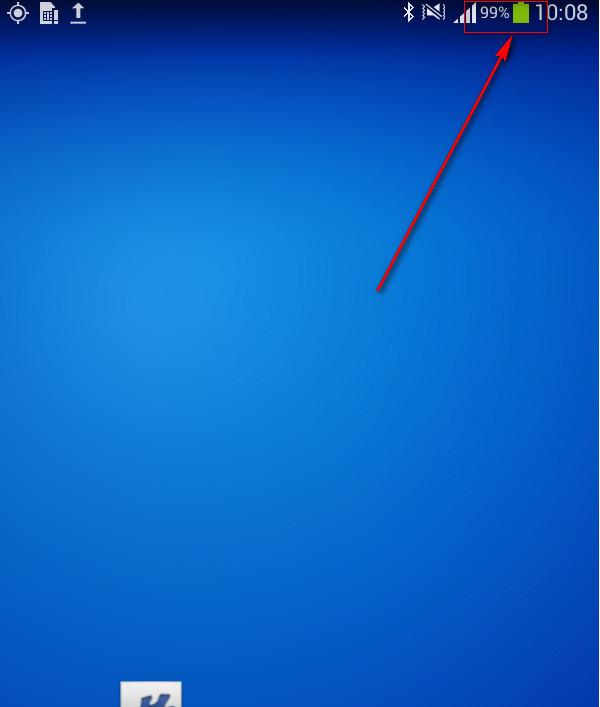
\includegraphics[width=0.5\linewidth]{scr1.jpg}}
		\ffigbox{\caption{Значок GPS}\label{pic:pic2}}%
		{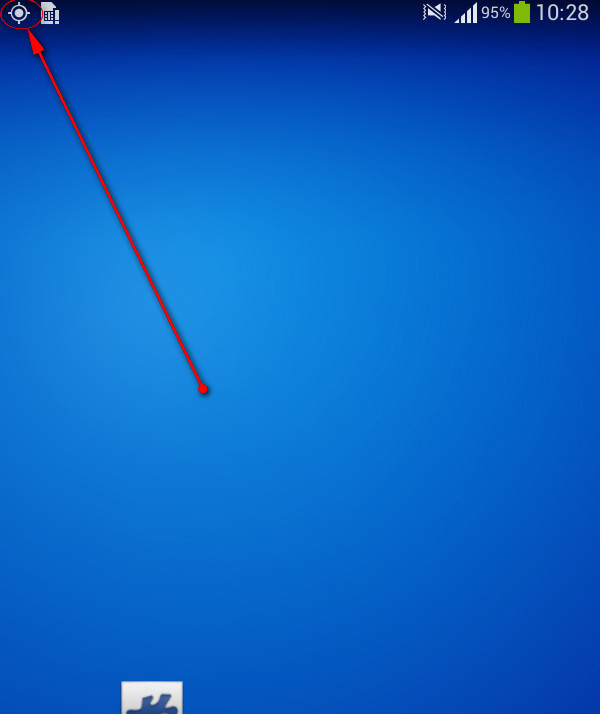
\includegraphics[width=0.5\linewidth]{scr2.jpg}}         
	\end{floatrow}
\end{figure}

Уровень заряда планшета в общем случае можно определить по значку «батарейки» расположенному в правом верхнем углу экрана.(рис.\ref{pic:pic1})
%\hyperref[pic:pic1]{рис.}
\item Затем торговый представитель должен определить включён ли у планшета модуль GPS.
При включённом модуле GPS  на самой верхней строчке экрана планшета, отображается значок GPS
(рис.\ref{pic:pic2})
\item После этого необходимо запустить программу «Оптимум» иконка которой расположена на рабочем столе планшета торгового представителя.Запуск программы осуществляется путём «тапа»(прикосновения к иконке программы).
(рис.\ref{pic:pic3})
\begin{figure}[h]
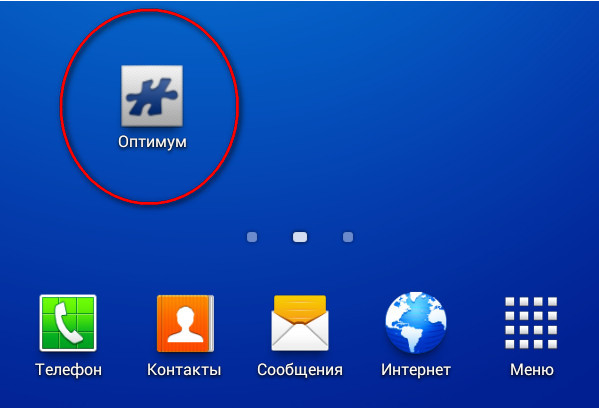
\includegraphics[width=0.3\linewidth]{scr3.jpg} 
\caption{<<Иконка>> Оптимы}\label{pic:pic3}
\end{figure}

\item При запуске программы пользователь попадает в главное меню <<Оптимы>>\label{it:it2_1}
(рис.\ref{pic:picgl})
\begin{figure}[h]
	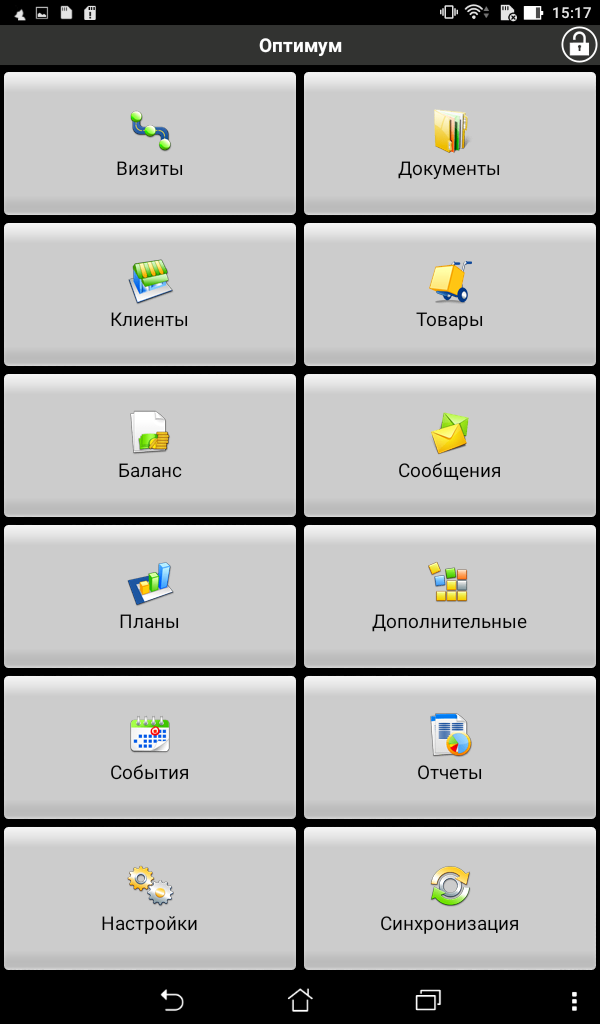
\includegraphics[width=0.2\linewidth]{scr_gl.png} 
	\caption{Главное меню <<Оптимы>>}\label{pic:picgl}
\end{figure}


\item Далее торговый представитель нажимает кнопку «Синхронизация»(рис.\ref{pic:pic4})
и попадает в раздел «Синхронизация».
(рис.\ref{pic:pic5})
\begin{figure}[h]
  \begin{floatrow}
   \ffigbox{\caption{Меню синхронизация}\label{pic:pic4}}%
           {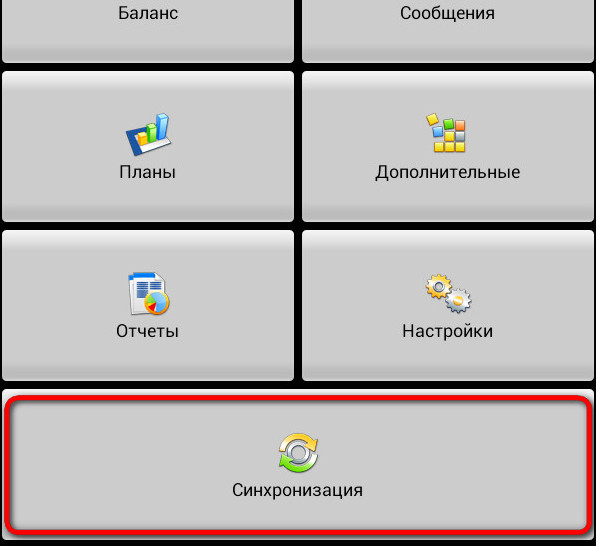
\includegraphics[width=0.8\linewidth]{scr4.jpg}}
   \ffigbox{\caption{Раздел синхронизация}\label{pic:pic5}}%
           {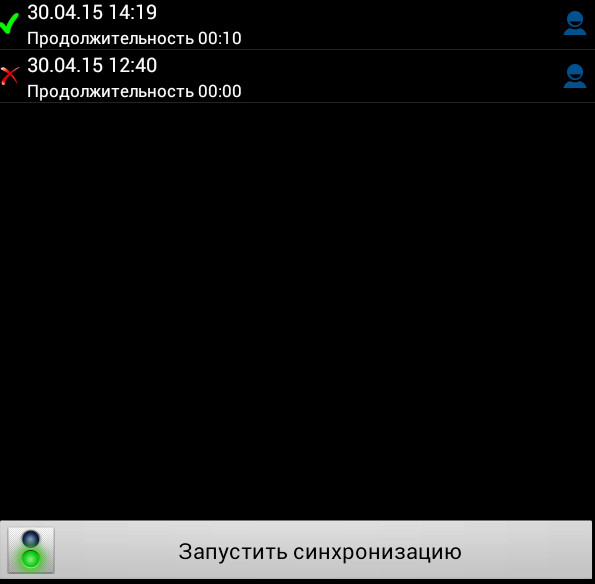
\includegraphics[width=0.75\linewidth]{scr5.jpg}}         
  \end{floatrow}
\end{figure}
%http://mydebianblog.blogspot.ru/2013/06/floatrow-figures-in-a-row.html
%http://mydebianblog.blogspot.ru/2013/06/floatrow-caption-position.html
\item В этом разделе торговый представитель, используя кнопку «Запустить синхронизацию» \label{it:it2_2}
(рис.\ref{pic:pic6})
совершает запуск синхронизации и дожидается ее окончания.(рис.\ref{pic:pic7}) 
\begin{figure}[!h]
	\begin{floatrow}
		\ffigbox{\caption{Запуск синхронизации}\label{pic:pic6}}%
		{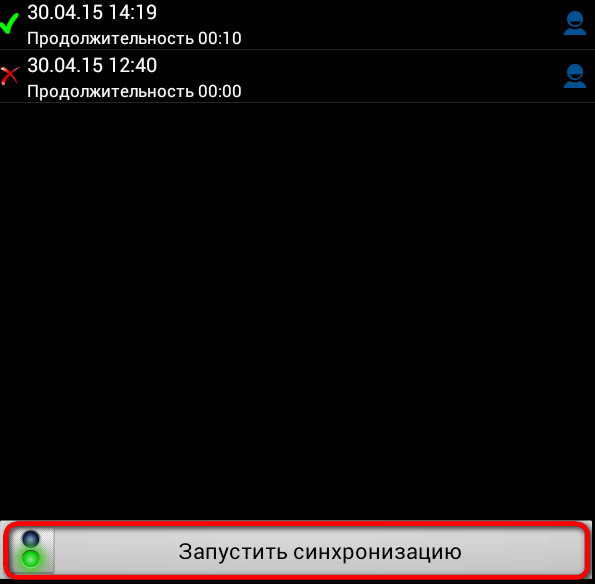
\includegraphics[width=0.8\linewidth]{scr6.jpg}}
		\ffigbox{\caption{Процесс синхронизации}\label{pic:pic7}}%
		{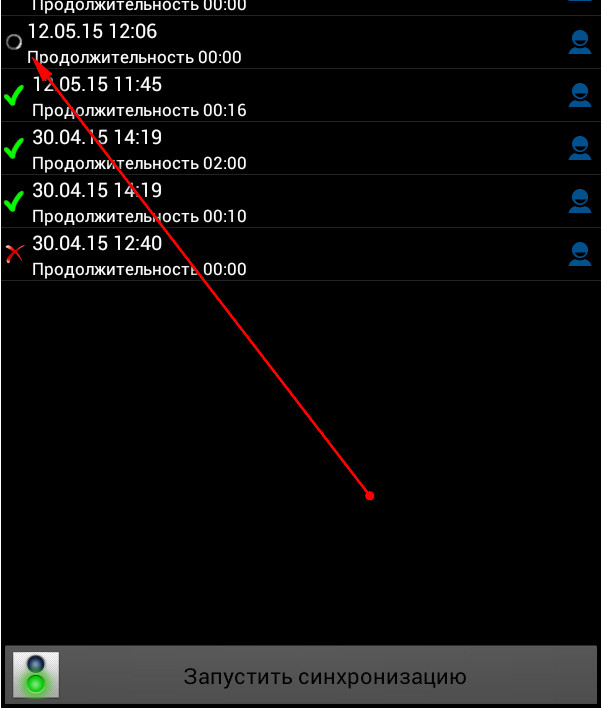
\includegraphics[width=0.75\linewidth]{scr7.jpg}}         
	\end{floatrow}
\end{figure}

Об успешном прохождении синхронизации свидетельствует «зелёная галочка» слева от строки с выполнявшейся синхронизацией.(рис.\ref{pic:pic8}) 
\begin{figure}[!h]
	\begin{floatrow}
		\ffigbox{\caption{Синхронизация успешна}\label{pic:pic8}}%
		{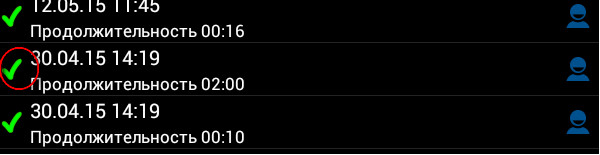
\includegraphics[width=0.8\linewidth]{scr8.jpg}}
		\ffigbox{\caption{Синхронизация неудачна}\label{pic:pic9}}%
		{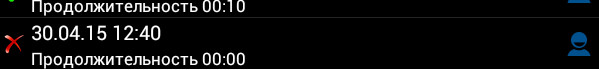
\includegraphics[width=0.75\linewidth]{scr9.jpg}}         
	\end{floatrow}
\end{figure}
\item Если отображается значок «красный крестик» (рис.\ref{pic:pic9}) это означает, что синхронизация «не прошла». 
В таком случае необходимо удостовериться, что на планшетном ПК включена  передача «мобильные данные» и повторить синхронизацию согласно  п. \ref{it:it2_2}
\item Если несколько раз подряд выполнение синхронизации не было успешным, необходимо «перезагрузить» планшет. Т.е. выключить его и повторно включить спустя 2-3 минуты. Затем повторить пункты с \ref{it:it2_1} по \ref{it:it2_2}
\item После этих действий планшетный ПК готов к работе.
\end{enumerate}% Последовательность работы торгового представителя с планшетным устройством
\section{Работа в торговой точке}
%\setcounter{figure}{0}
\begin{enumerate}[\thesection .1]
\item Подъехав к торговой точке, торговый представитель в программе «Оптимум» нажимает кнопку «Визиты» 
(рис.\ref{pic:pic10})

\begin{figure}[!h]
	\begin{floatrow}
		\ffigbox{\caption{Визиты}\label{pic:pic10}}%
		{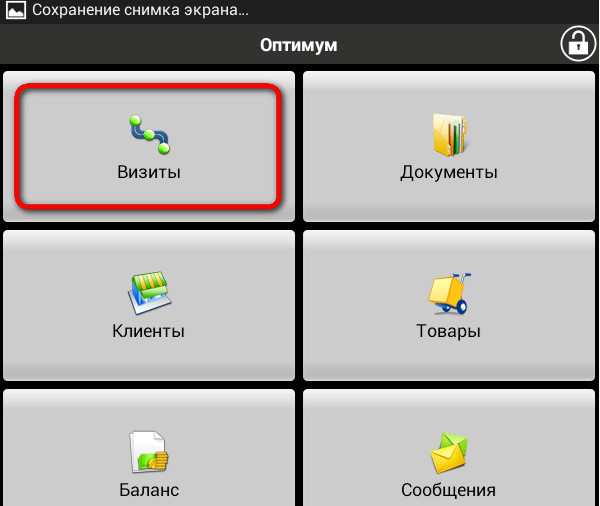
\includegraphics[width=0.8\linewidth]{scr10.jpg}}
		\ffigbox{\caption{Выбор торговой точки}\label{pic:pic11}}%
		{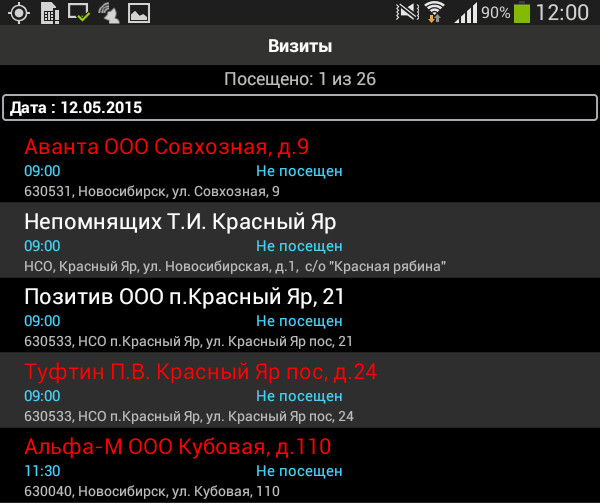
\includegraphics[width=0.8\linewidth]{scr11.jpg}}         
	\end{floatrow}
\end{figure}
\item Торговый представитель попадает в раздел «Визиты»
\footnote{Раздел «Визиты» предназначен для работы с маршрутами торгового представителя. "Визит" в системе "Оптимум" нужно рассматривать как факт посещения торговой точки за дату.} программы «Оптимум»
%То есть, несмотря на то, что фактически торговый представитель мог за день посетить данную ТТ несколько раз, в Системе будет зафиксирован один визит в данную ТТ (независимо от числа созданных документов и количества сеансов синхронизации с сервером).
(рис.\ref{pic:pic11}) и может выбрать необходимую торговую точку.
(подробно о визитах см.раздел\ref{sec:sec14_1})

Маршрут - это список посещений (визитов) клиентов торговым представителем на текущую дату. У мобильного сотрудника имеется возможность создать внеплановый визит в ТТ.
(см.\ref{sec:sec11_1})

\item Далее торговый представитель выбирает нужную ТТ, выполняет  «длительное нажатие»  (порядка 1-1,5 сек) и в открывшемся меню выбирает «Изменить статус»\label{it:it1}
(рис.\ref{pic:pic12})
\begin{figure}[!h]
\begin{floatrow}
	\ffigbox{\caption{Изменение статуса}\label{pic:pic12}}%
	{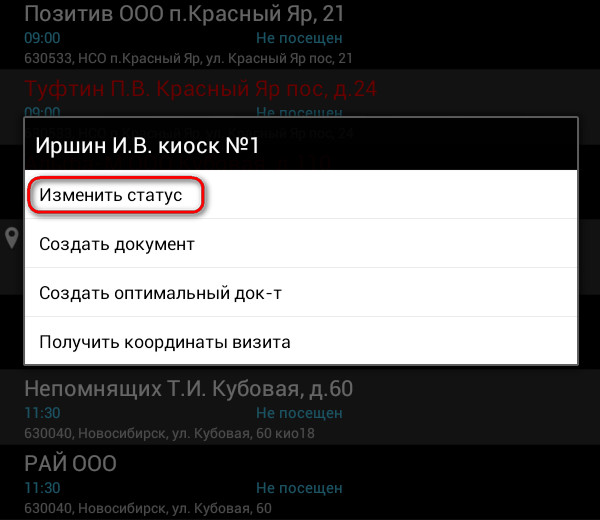
\includegraphics[width=0.8\linewidth]{scr12.jpg}}
	\ffigbox{\caption{Начало визита}\label{pic:pic13}}%
	{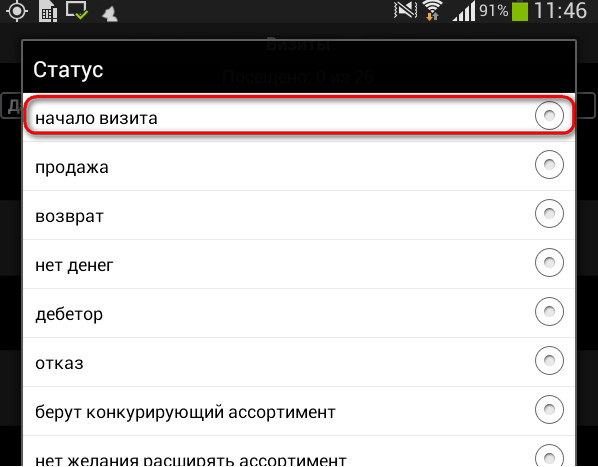
\includegraphics[width=0.8\linewidth]{scr13.jpg}}         
\end{floatrow}
\end{figure}
\item В следующем открывшемся меню выбирает «начало визита»\label{it:it2} 
(рис.\ref{pic:pic13})
\item Далее торговый представитель вновь выбирает нужную ТТ, выполняет  «длительное нажатие»  и в открывшемся меню выбирает «Получить координаты визита» . В случае если  и спутники обнаружены, текущие GPS-координаты торговой точки будут записаны в базу данных Мобильной части. Занимает данная процедура по времени не более 25 сек.\label{it:it3}
(рис.\ref{pic:pic14})
\begin{figure}[!h]
	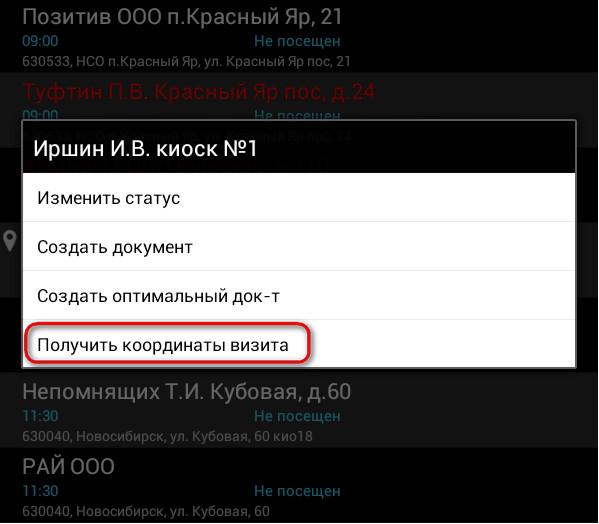
\includegraphics[width=0.4\linewidth]{scr14.jpg} 
	\caption{Получение координат визита}\label{pic:pic14}
\end{figure}

\item Когда координаты получены верно, на экране планшета рядом с наименованием ТТ в маршрутном листе слева сбоку должен появиться символ «капли»(1) ,его наличие говорит о том, что координаты визита получены и можно начинать работу. Так же изменился статус визита (2).
В противном случае если координаты визита получить не удалось, на экране будет появляться сообщение о том , что «координаты определить не удалось» в таком случае  повторяем пункт \ref{it:it2_1}
(рис.\ref{pic:pic15})
\begin{figure}[!h]
	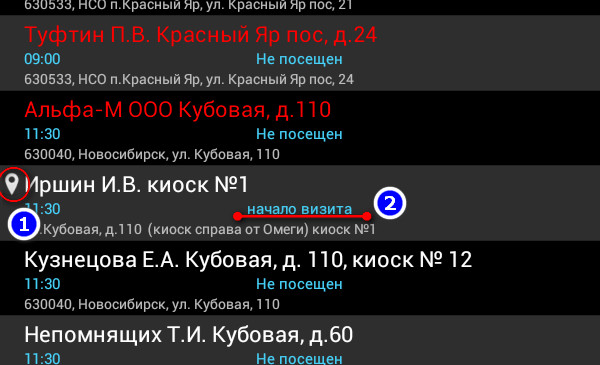
\includegraphics[width=0.5\linewidth]{scr15.jpg} 
	\caption{Координаты визита получены}\label{pic:pic15}
\end{figure}
\item Если GPS модуль включён, но координаты так и не определяются, необходимо определить координаты после окончания визита в ТТ, находясь на улице непосредственно на территории ТТ. воспользовавшись пунктом \ref{it:it2_1}

\item Затем торговый представитель заходит непосредственно в точку и выполняет там необходимые действия

\item \label{sec:sec3_1} Торговый представитель оформляет заказ. Для этого необходимо выполнить «длительное нажатие»  на ТТ с которой происходит работа  и из появившегося меню выбрать пункт «Создать документ»
(рис.\ref{pic:pic17})
\begin{itemize}
\item Выбрать тип создаваемого документа и произвести с ним необходимую работу.
(рис.\ref{pic:pic18})
\begin{figure}[!h]
	\begin{floatrow}
		\ffigbox{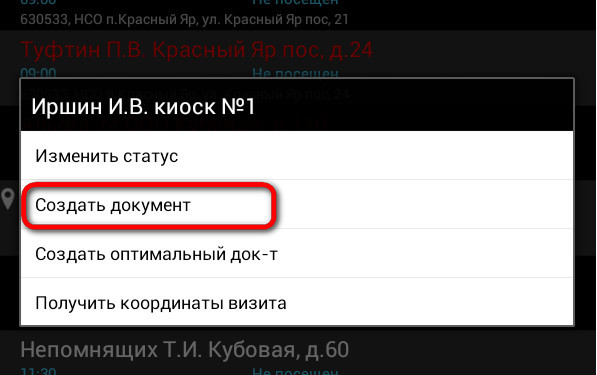
\includegraphics[width=0.9\linewidth]{scr17.jpg}}%
		{\caption{Создание документа}\label{pic:pic17}}
		\ffigbox{\caption{Выбор типа документа}\label{pic:pic18}}%
		{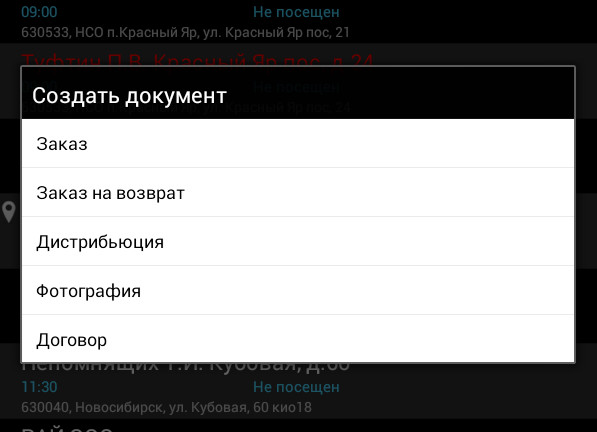
\includegraphics[width=0.8\linewidth]{scr18.jpg}}         
	\end{floatrow}
\end{figure}
\item Открывается окно просмотра заголовка документа.Вид и состав данных в окне заголовка документа зависит от типа документа, с которым идет работа в текущий момент. Помимо полей заголовка документа в этом окне так же отображаются атрибуты документа. 
В заголовке документа может быть не выбран <<тип оплаты>>.
(рис.\ref{pic:pic20})
\begin{figure}[!h]
	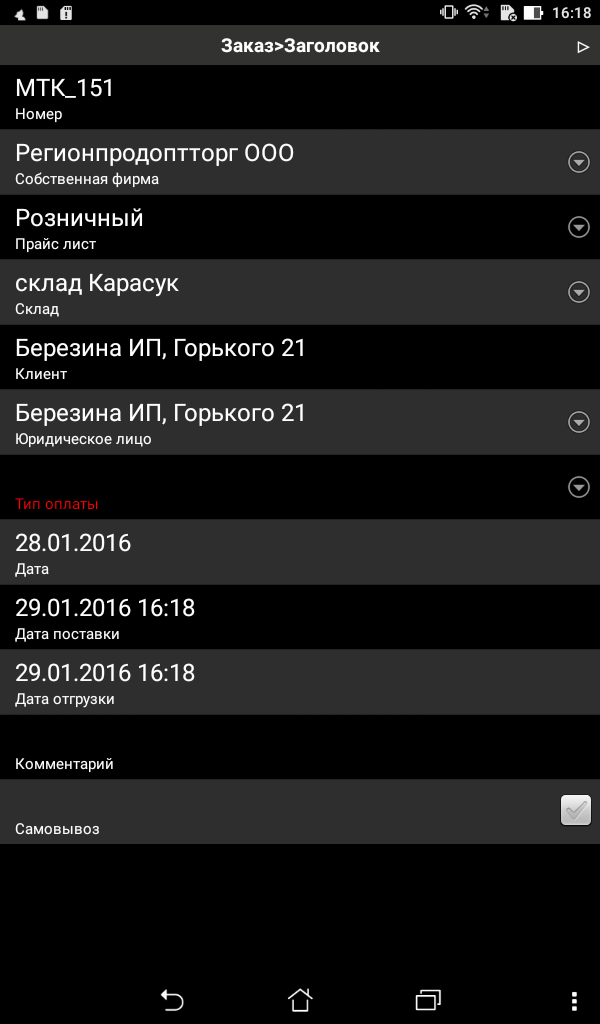
\includegraphics[width=0.25\linewidth]{scr20.png} 
	\caption{Шапка документа}\label{pic:pic20}
\end{figure}

\item Выбирается необходимый тип оплаты, если он не выбран.
(рис.\ref{pic:pic21})
\item Теперь шапка документа с заполненным типом оплаты. Необходимо нажать стрелку вправо (1), либо нужно совершить скользящее касание экрана слева – направо. 
Это позволит перейти к заполнению документа.
(рис.\ref{pic:pic22})
\begin{figure}[!h]
	\begin{floatrow}
		\ffigbox{\caption{Возможные типы оплаты}\label{pic:pic21}}%
		{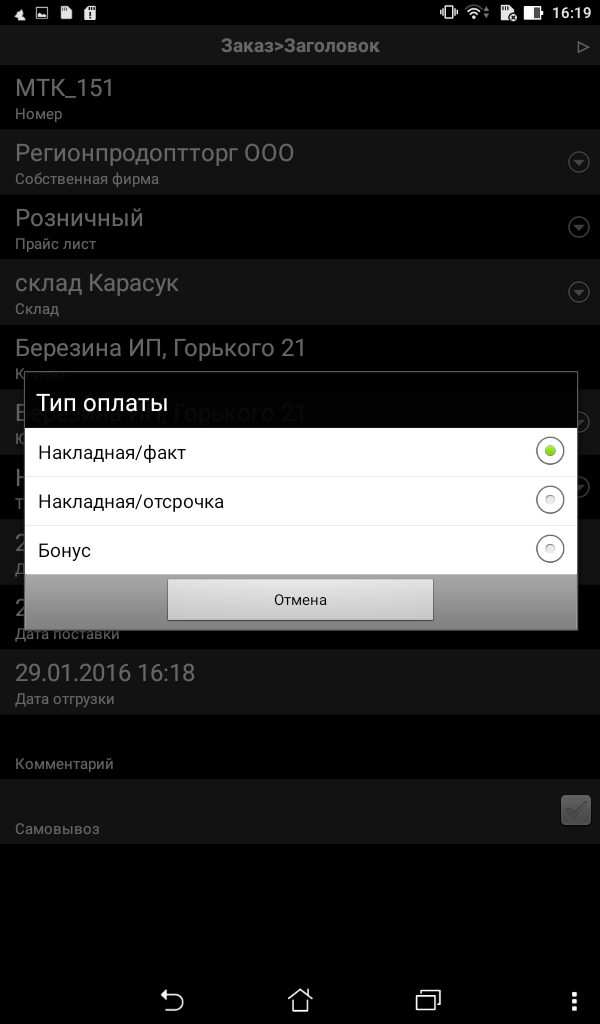
\includegraphics[width=0.6\linewidth]{scr21.png}}
		\ffigbox{\caption{Шапка документа с типом оплаты}\label{pic:pic22}}%
		{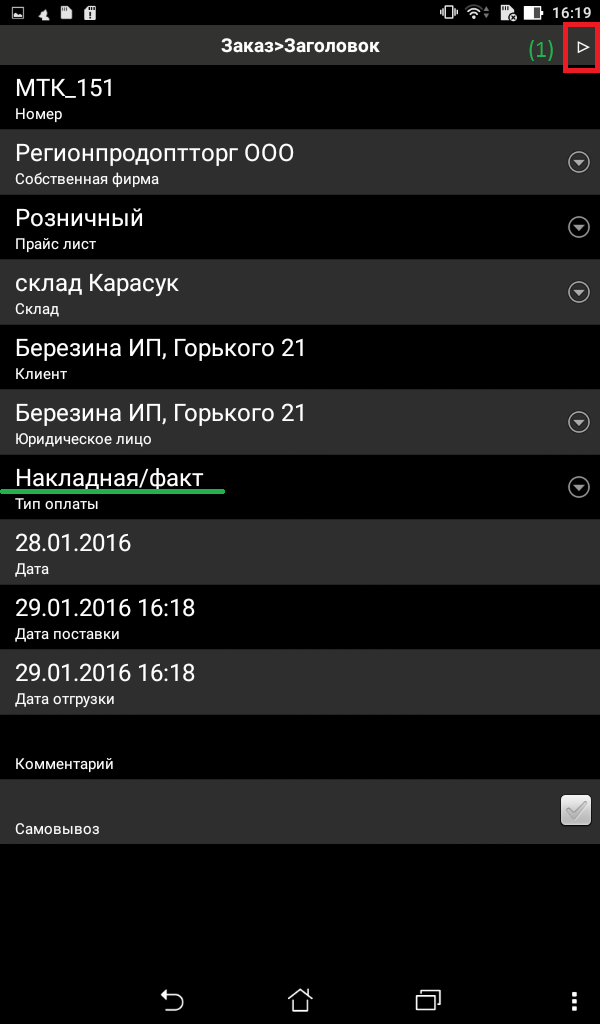
\includegraphics[width=0.6\linewidth]{scr22.png}}         
	\end{floatrow}
\end{figure}

\item Окрывается документ.
(рис.\ref{pic:pic23})
Экран с позициями может незначительно видоизменяться в зависимости от типа документа.В списке позиций присутствуют дополнительные справочные данные по позиции, такие как остаток на центральном складе и цена. 
При удержании элемента осуществляется переход к форме просмотра детальной информации о товарах. 
%\begin{figure}[h!]
%	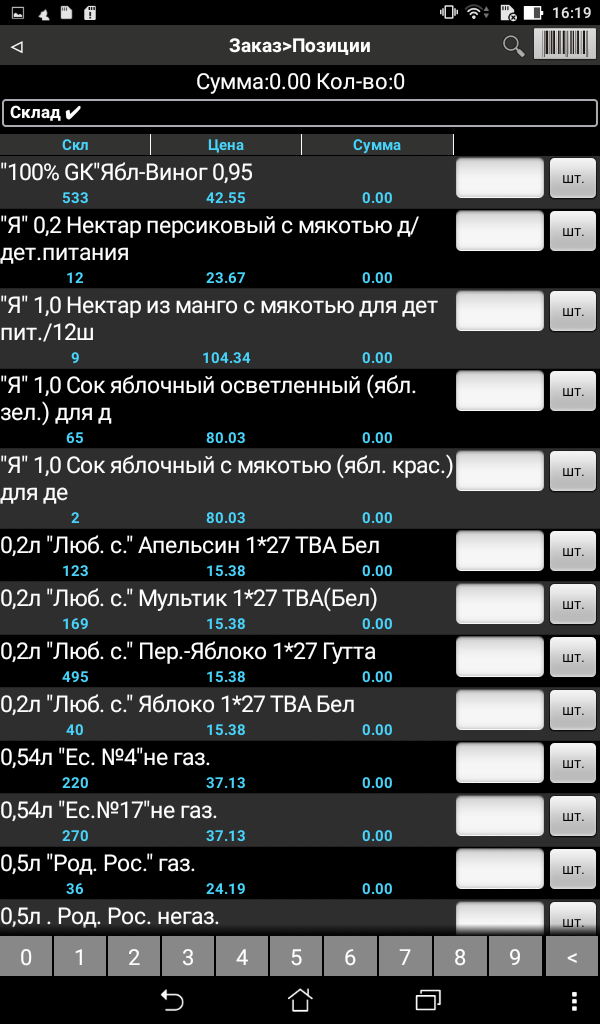
\includegraphics[width=0.3\linewidth]{scr23.png} 
%	\caption{Документ}\label{pic:pic23}
%\end{figure}
\item Далее в документе выбираются нужные позиции и проставляются количества товара.
(рис.\ref{pic:pic24})
\item Если всё сделано правильно, то при закрытии документа, на запрос, выбираем <<сохранить>>.
(рис.\ref{pic:pic25})
\begin{figure}[!h]
	\begin{floatrow}[3]
		\ffigbox{\caption{Документ}\label{pic:pic23}}%
		{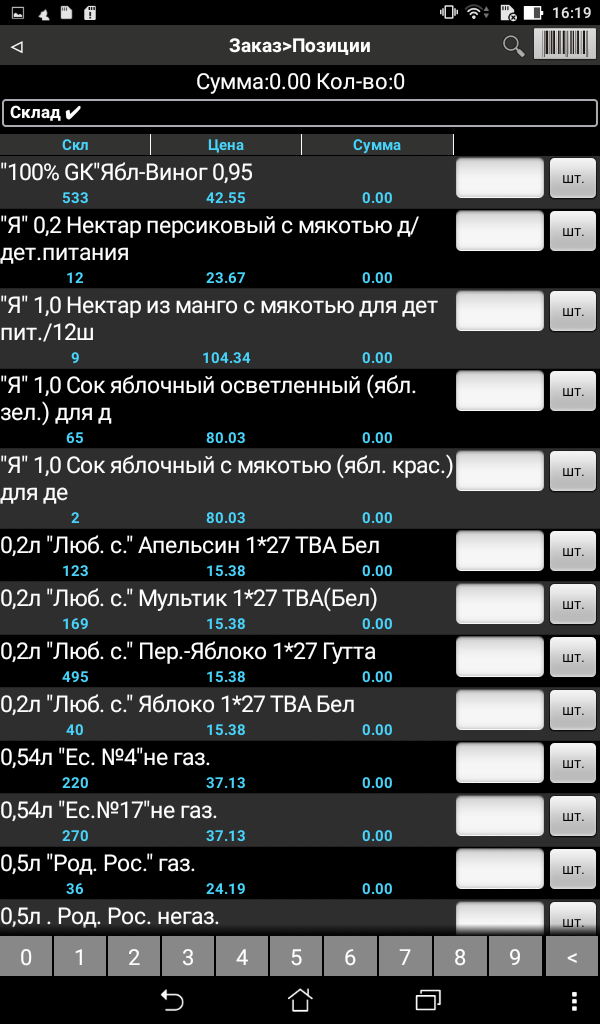
\includegraphics[width=0.8\linewidth]{scr23.png}}
		\ffigbox{\caption{Заполнение документа}\label{pic:pic24}}%
		{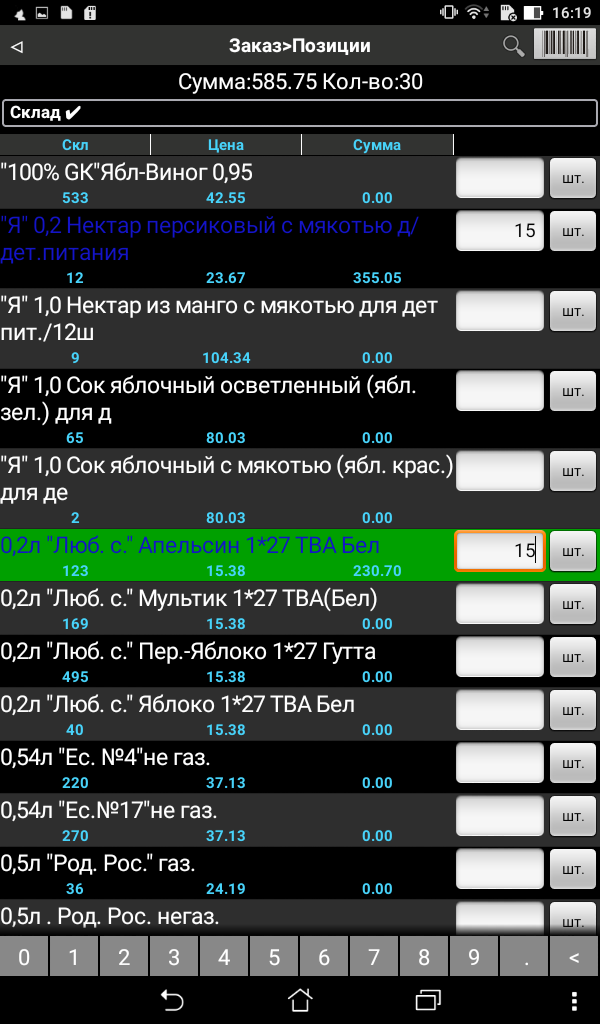
\includegraphics[width=0.8\linewidth]{scr24.png}}
		\ffigbox{\caption{Закрытие документа}\label{pic:pic25}}%
		{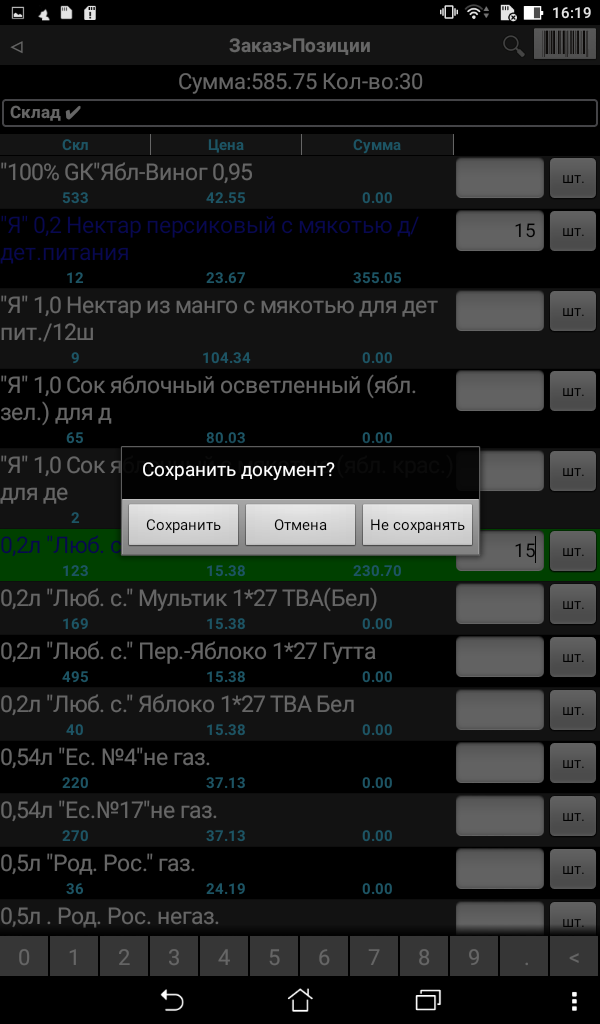
\includegraphics[width=0.8\linewidth]{scr25.png}}         
	\end{floatrow}
\end{figure}

\item Теперь созданный документ появится в списке документов.
(рис.\ref{pic:pic26})
\item Торговый представитель создаёт документ (рис.\ref{pic:pic18}) «Фотография»
и выполняет фотографирование  ассортимента представленного в ТТ.
(рис.\ref{pic:pic19})
\begin{figure}[!h]
	\begin{floatrow}
		\ffigbox{\caption{Список документов}\label{pic:pic26}}%
		{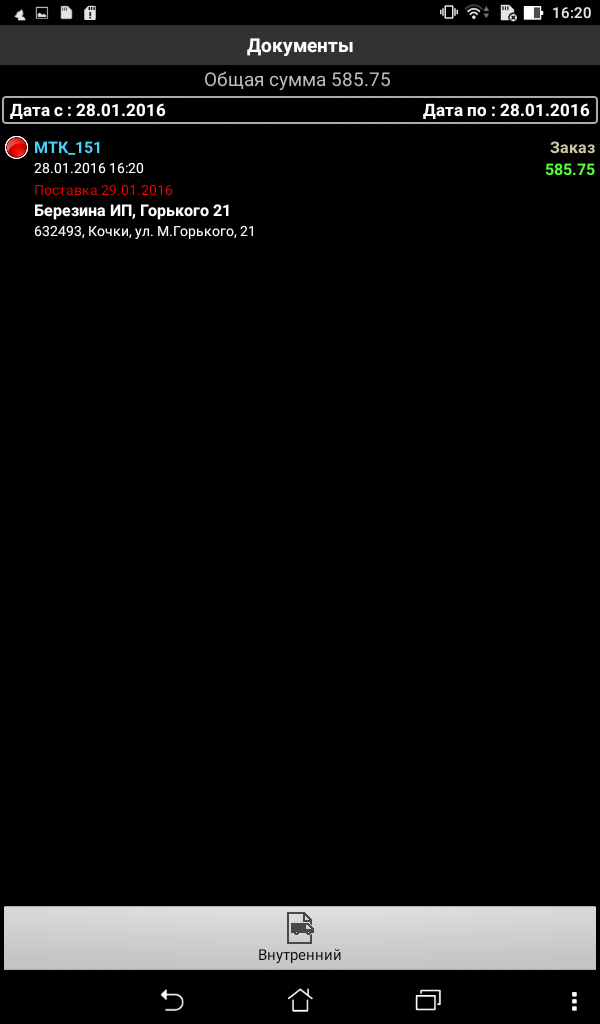
\includegraphics[width=0.6\linewidth]{scr26.png}}
		\ffigbox{\caption{Выбор типа для фотографии}\label{pic:pic19}}%
		{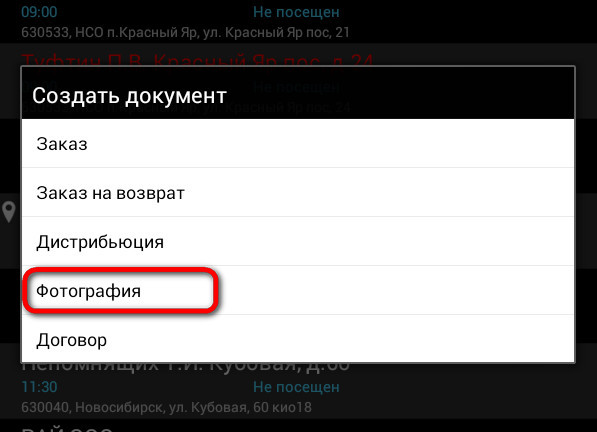
\includegraphics[width=0.8\linewidth]{scr19.jpg}}         
	\end{floatrow}
\end{figure}
\item Открывается документ «Фотография».Необходимо нажать стрелку вправо (1). Это позволит перейти к заполнению документа.
(рис.\ref{pic:pic27})
\item В открывшемся документе нажимаем кнопку <<добавить>>.
(рис.\ref{pic:pic29})
\begin{figure}[!h]
	\begin{floatrow}
		\ffigbox{\caption{Список документов}\label{pic:pic27}}%
		{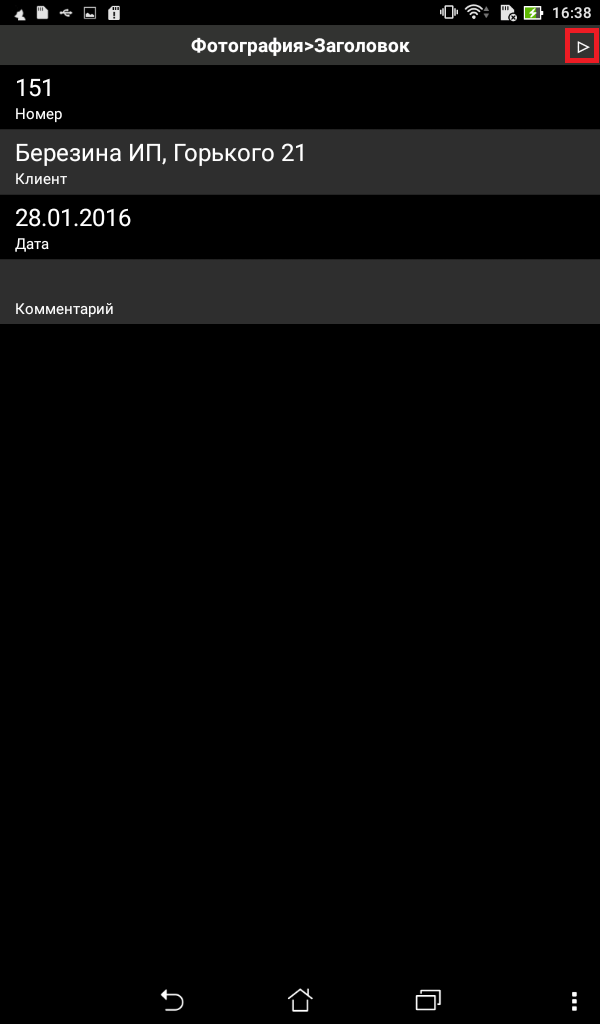
\includegraphics[width=0.6\linewidth]{scr27.png}}
		\ffigbox{\caption{Кнопка добавить фотографию}\label{pic:pic29}}%
		{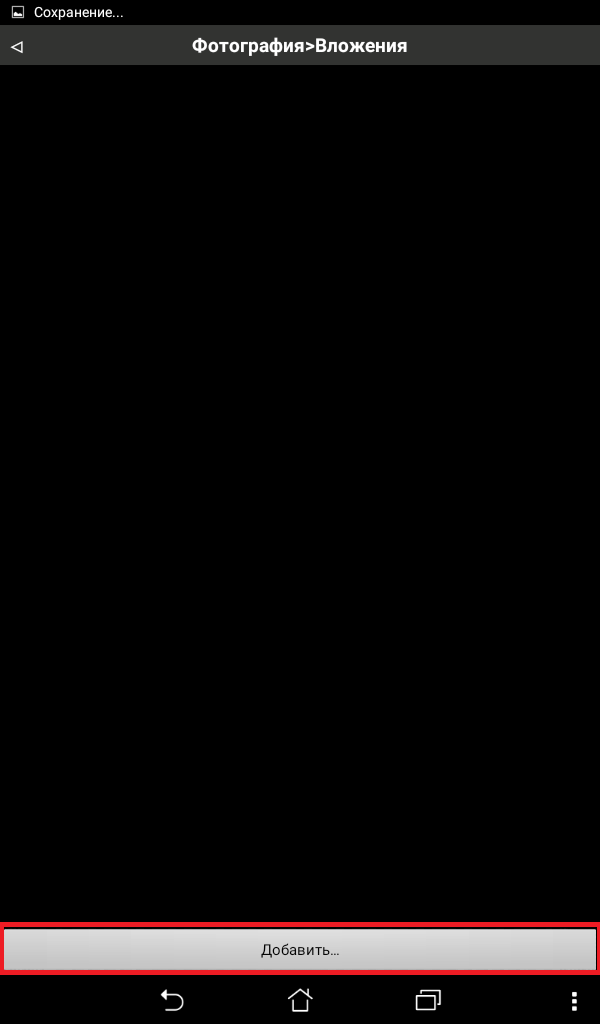
\includegraphics[width=0.6\linewidth]{scr29.png}}         
	\end{floatrow}
\end{figure}



\item КПК переходит в режим фотографирования. Выбираем необходимый план и фотографируем.
(рис.\ref{pic:pic30})
\begin{figure}[!h]
	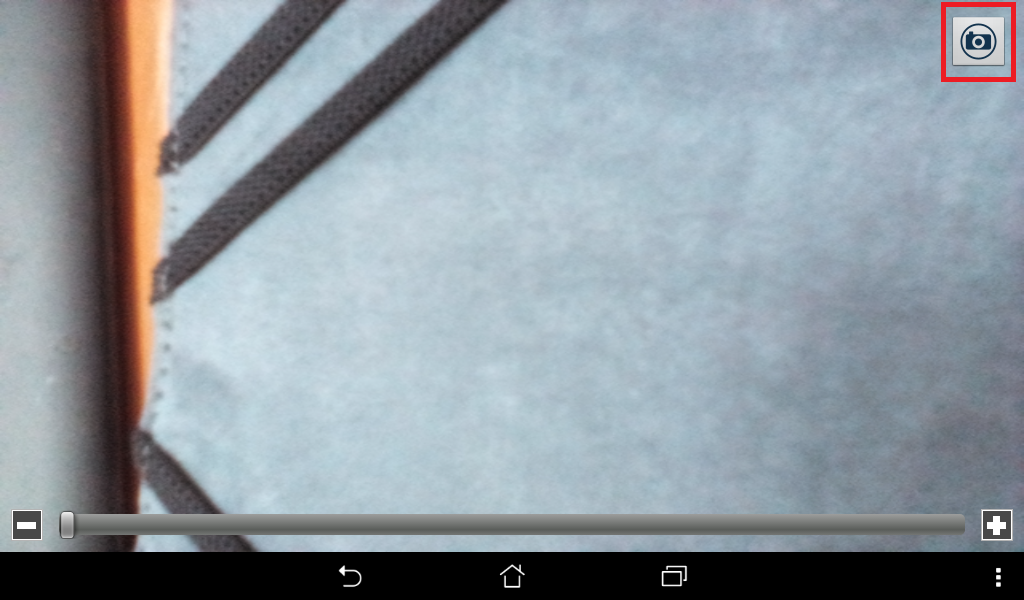
\includegraphics[width=0.5\linewidth]{scr30.png} 
	\caption{Фотография}\label{pic:pic30}
\end{figure}
\item Для прикрепления ещё одной фотографии выполните описанные действия снова (кнопка «Добавить…»)
\item Для удаления фотографии нажмите на файле соответствующей фотографии и в открывшемся окне нажмите на кнопку «Удалить».
\item Размер фотографий задаётся в модуле Настройки. 
  

\end{itemize}

\item По окончанию визита необходимо запустить процесс синхронизации описанный в п.\ref{it:it2_1} по \ref{it:it2_2}

\item В случае, если при посещении ТТ торговым представителем не был оформлен заказ для этой ТТ, агенту необходимо, находясь ещё на территории данной ТТ поменять статус посещения (п.\ref{it:it1}) ТТ на необходимый: «Дебитор», «Нет денег», «Товар в наличии» или иные причины.
\item Переход к определённой позиции документа\\
При формировании документа в момент ввода количественных данных по товарным позициям у сотрудника может возникнуть потребность в быстром переходе к той или иной товарной позиции в большом списке товаров. Для этого предусмотрена специальная функция, которую можно вызвать из общего меню, нажав на кнопку \textbf{Перейти к....} 

\includegraphics[width=0.03\linewidth]{scr_cm.png} 
После запуска функции перехода откроется окно выбора вариантов поиска: поиск по краткому наименованию объекта, по полному наименованию или по внешнему коду объекта. Выбрав наиболее подходящий вариант, необходимо в нижней части окна ввести символы, по которым будет вестись поиск конкретной товарной позиции.
\item Акцептование/разакцептование документа\\
В рамках Системы термин \textbf{Акцептование} означает перевод документа в состояние, в котором его редактирование или удаление недоступно пользователю. 
\item Удаление документа\\
В мобильной части Системы предусмотрено удаление акцептованных и неакцептованных документов, которые не были переданы в серверную часть. Неакцептованные документы всегда доступны для удаления.Документы, переданные в серверную часть недоступны для удаления в любом случае.
Для того чтобы удалить документ, выполните следующие действия:
\begin{itemize}
	\item В модуле \textbf{Документы} выберите документ и откройте его контекстное меню;
	\item В контекстном меню выберите пункт \textbf{Удалить документ};
\end{itemize}
Выбранный документ будет удален.
\end{enumerate}% Работа в торговой точке
%\section{Предоставление отчета о деятельности торгового агента.}
Аналитик – координатор отдела прямых продаж ООО «Регионпродоптторг» на ежедневной основе, по факту окончания рабочего дня торгового представителя (до 18:00 текущего дня)  формирует «Отчёт о деятельности агента» с программы 1С ООО «Регионпродоптторг» за текущий день (форма документа в Приложении № 1 к настоящему Регламенту) и направляет данный сформированный отчёт на электронный адрес следующим лицам:
\begin{itemize}[topsep=0pt, itemsep=-0.5ex]
	\item Супервайзеру отдела городских продаж ООО «Торговый Дом «Солнечные Продукты».
	\item Региональному менеджеру по продажам ООО «Торговый Дом «Солнечные продукты».
\end{itemize}

%\section{Нарушения торговых представителей, отражаемых в «Отчёте о нарушениях торговых агентов, работающих по контракту «Новосибирский жировой комбинат».}
\begin{enumerate}[\thesection .1]
\item Аналитик – координатор отдела прямых продаж ООО «Регионпродоптторг» на ежедневной основе, по факту окончания рабочего дня торгового представителя, работающего по контракту «Новосибирский жировой комбинат» формирует «Отчёт о работе торговых агентов» (форма документа в Приложении № 2 к настоящему Регламенту). В данном отчете указываются следующие виды нарушений:	

\item Количество не посещённых торговых точек торговым представителем (отсутствие визита в торговую точку), согласно маршрутного листа.

\item Время начала рабочего дня торгового агента (согласно данным GPRS), а именно, посеще-ние первой торговой точки согласно маршрутному листу, в 10:00. 

\item Время окончания рабочего дня торгового агента (согласно данным GPRS), а именно, посе-щение последней торговой точки согласно маршрутному листу, в 16:30.

\item В случае выявления хотя бы одного из видов нарушений (п. 4.1 настоящего Регламента) торго-вым представителем по контракту «Новосибирский жировой комбинат», данный торговый представи-тель должен предоставить объяснительную записку о причине нарушения. Объяснительная записка оформляется на имя Директора подразделения ООО «Регионпродоптторг». 

Если причина нарушения отсутствует или является не уважительной, то работодатель вправе не учитывать рабочий день, когда было допущено нарушение, в табеле учёта рабочего времени торго-вых представителей.	
\end{enumerate}

%\section{Предоставление табеля учёта рабочего времени по торговым представителям, работающим по контракту «Новосибирский жировой комбинат».}
\begin{enumerate}[\thesection .1]
\item Табель учёта рабочего времени за отчётный период (месяц) торговых представителей, работающих по контракту «Новосибирский жировой комбинат» (форма документа в Приложении № 3 к настоящему Регламенту) заполняется аналитиком-координатором ООО «Регионпродоптторг» в соответствии с учётом нарушений торговых агентов за каждый рабочий день отчётного месяца, а соответственно, с учётом зачтённого/незачтённого рабочего дня торгового представителя за соответствующий рабочий день. 
 5.2 Табель учета рабочего времени в обязательном порядке согласованный следующими лицами:
 - Директор подразделения ООО «Регионпродоптторг» (г. Новосибирск и НСО).
 - И.О. директора по продажам ООО «Регионпродоптторг» (г. Новосибирск).
 - Аналитик «Отдела прямых продаж» ООО «Регионпродоптторг» (г. Новосибирск). 
 - Региональный менеджер по продажам ООО ТД «Солнечные Продукты».

 5.3  После подписания всеми участниками (п.5.2 настоящего Регламента), табель учёта рабочего времени торговых представителей, работающих по контракту «Новосибирский жировой комбинат» предоставляется аналитиком-координатором «Отдела прямых продаж» руководителю отдела по работе с персоналом ООО «Регионпродоптторг» ежемесячно, в следующие сроки:
 - 16-ого числа отчетного месяца предоставляется табель за 15 дней отчетного мес.;
 - 1-ого числа месяца, следующего за отчётным, предоставляется табель за 30/31 день отчетного ме-сяца. 
 
\end{enumerate}	
\section{Дебиторка}
\begin{enumerate}[\thesection .1]
	\item Для просмотра дебиторской задолжности необходимо находясь в главном меню <<Оптимы>> (рис.\ref{pic:picgl}). Выбрать пункт <<Баланс>>
	(рис.\ref{pic:pic5_1})
	\item Открывается список баланса контрагентов. %Контрагенты имеющие просроченную задолжность
	 %отображаются красным цветом.	
	 (рис.\ref{pic:pic5_2})
	\item При длительном нажатии на надпись с контрагентом, открывается подробный список задолжностей с документами.	
	(рис.\ref{pic:pic5_3})	 
	 \begin{figure}[!h]
	 	\begin{floatrow}[3]
	 		\ffigbox{\caption{Просмотр баланса}\label{pic:pic5_1}}%
	 		{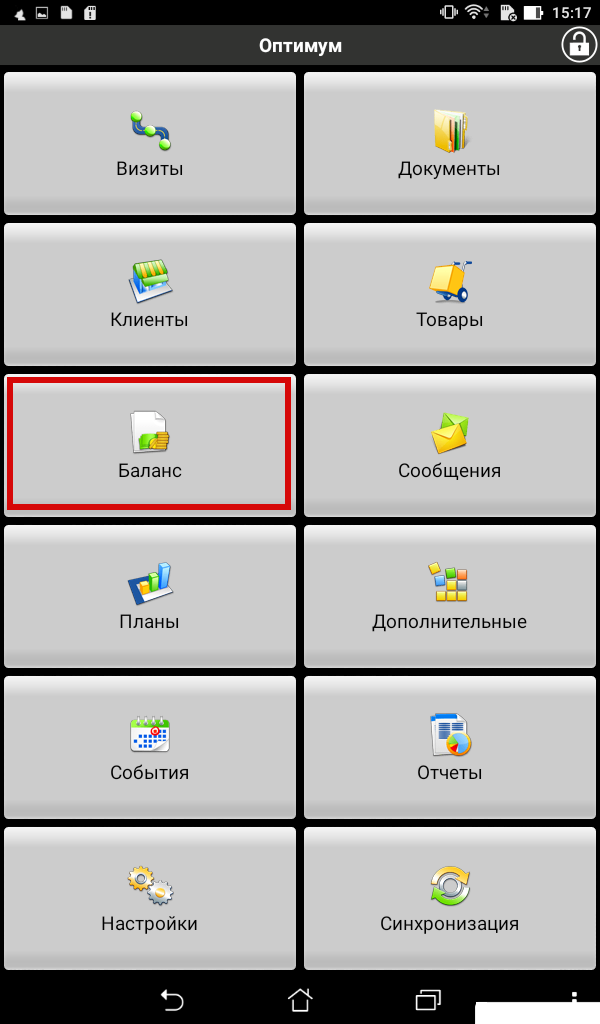
\includegraphics[width=0.8\linewidth]{scr5_1.png}}
	 		\ffigbox{\caption{Баланс}\label{pic:pic5_2}}%
	 		{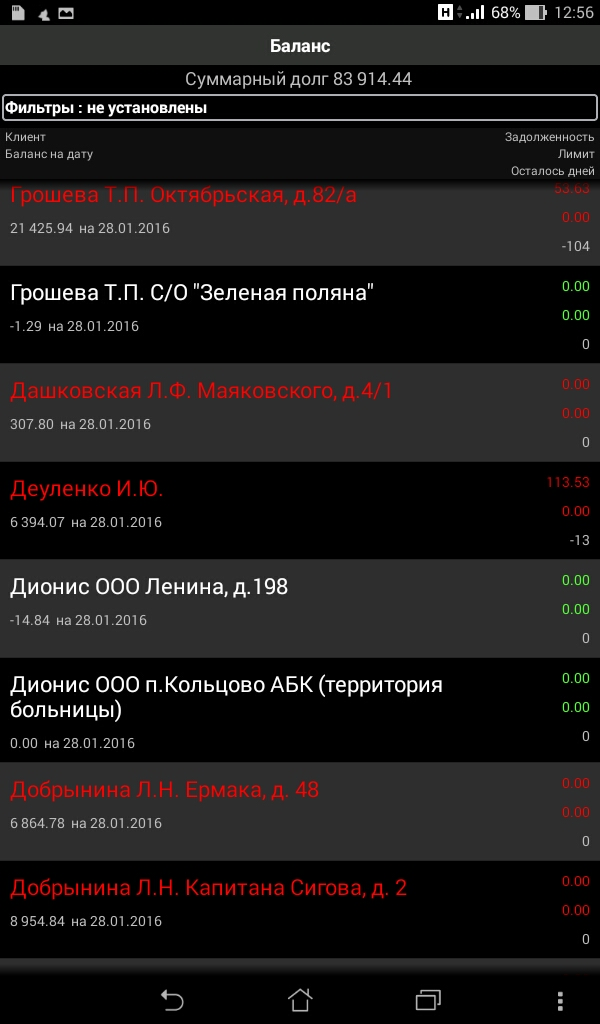
\includegraphics[width=0.8\linewidth]{scr5_2.jpg}}         
	 		\ffigbox{\caption{Подробный баланс}\label{pic:pic5_3}}%
	 		{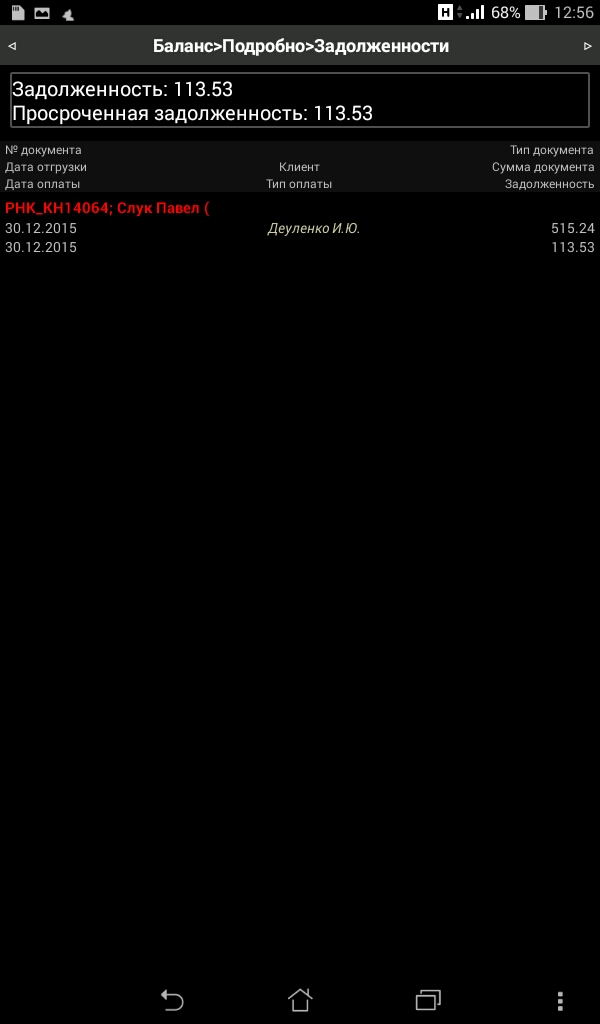
\includegraphics[width=0.8\linewidth]{scr5_3.jpg}}    
	 	\end{floatrow}
	 \end{figure}
	 
		
		
		

\end{enumerate}% Дебиторка
\section{Полная синхронизация}
\begin{enumerate}[\thesection .1]
	\item Находясь в меню <<Синхронизация>> (рис.\ref{pic:pic5}). Необходимо нажать кнопку дополнительного меню внизу экрана планшета. На разных планшетных ПК эта кнопка может выглядеть по разному. В общем случае она обозначается как три точки или три линии.
	После нажатия появится возможность выбрать тип синхронизации
	(рис.\ref{pic:pic9_1})
	\begin{figure}[!h]
		\begin{floatrow}
			\ffigbox{\caption{Выбор типа синхронизации}\label{pic:pic9_1}}%
			{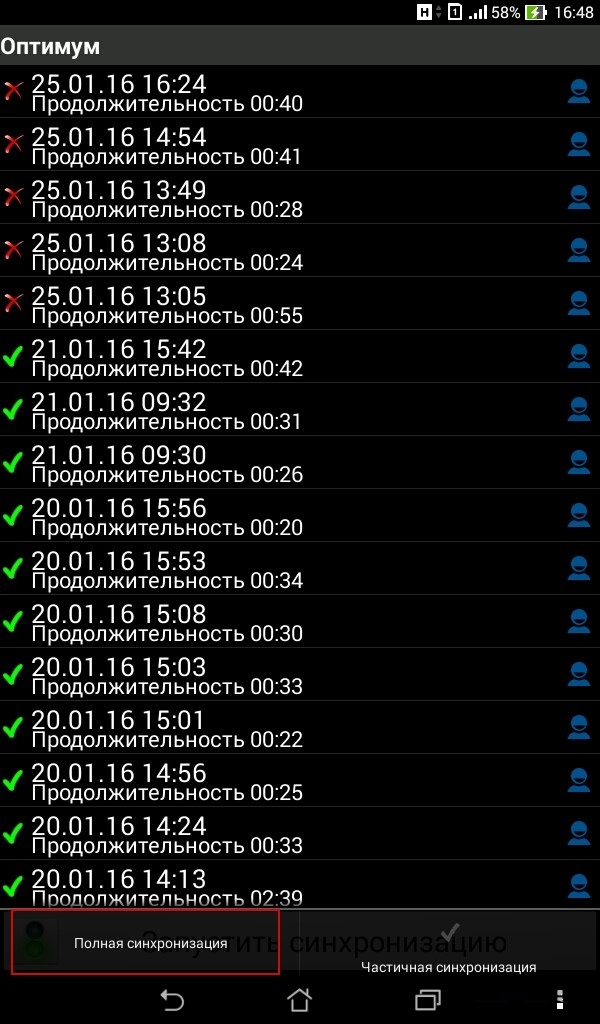
\includegraphics[width=0.8\linewidth]{scr9_1.jpg}}
		\end{floatrow}
	\end{figure}
	Нужно отметить тип <<Полная синхронизация>>, а затем запустить синхронизацию
\end{enumerate}
% Полная синхронизация
\section{Ввод временных координат}
\begin{enumerate}[\thesection .1]
	\item Для получения "временных координат" торговой точки, необходимо находясь 
	(рис.\ref{pic:pic9_1})
	\begin{figure}[!h]
		\begin{floatrow}
			\ffigbox{\caption{Выбор типа синхронизации}\label{pic:pic9_1}}%
			{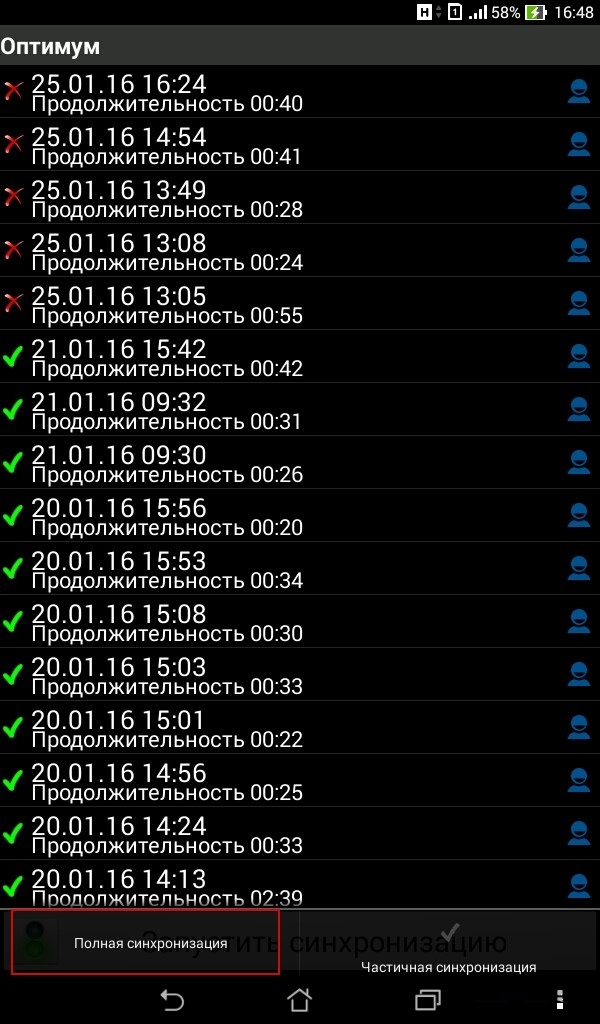
\includegraphics[width=0.8\linewidth]{scr9_1.jpg}}
		\end{floatrow}
	\end{figure}
	Нужно отметить тип <<Полная синхронизация>>, а затем запустить синхронизацию
\end{enumerate}	% Ввод временных координат
\section{Закрытие программы}
\begin{enumerate}[\thesection .1]
	\item В главном меню <<Оптимы>> (рис.\ref{pic:picgl}) в правом верхнем углу можно заметить значок <<Замочек>>.(1) В нормальном состоянии он слегка приоткрыт. Это говорит о том, что с системой можно работать.(рис.\ref{pic:pic7_1})
    При закрытии программы стандартными средствами Android с помощью стрелки назад выводится следующее сообщение о том что при выходе из программы будет произведено закрытие дня. Если выбрать утвердительный ответ,то программа закроется и при следующем открытии <<Замочек>> будет закрыт и никакие действия в программе невозможны. Для решения этой проблемы необходимо звонить в отдел IT или своему непосредственному руководителю.
    \begin{figure}[H]
    	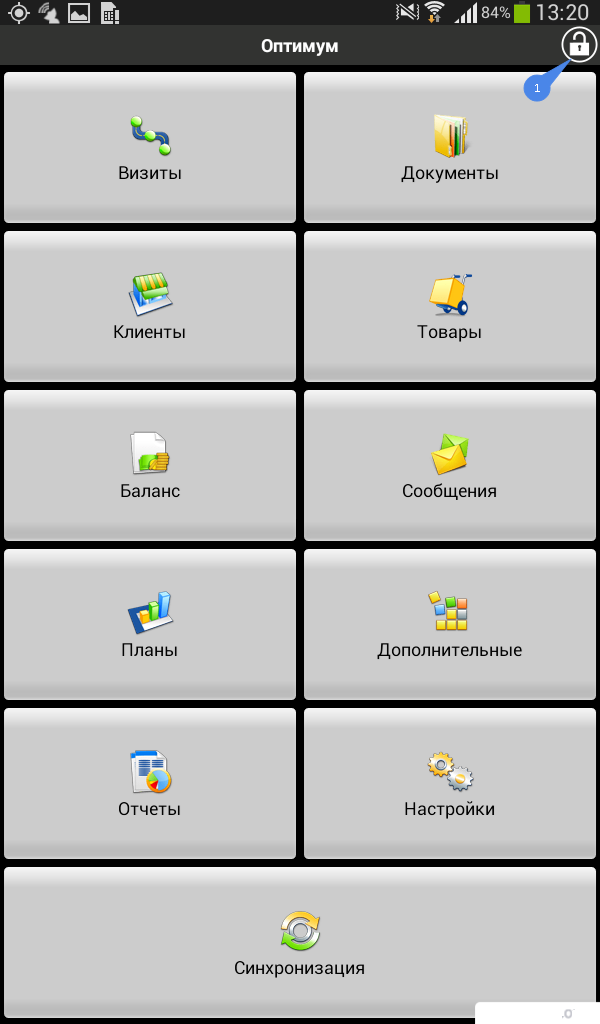
\includegraphics[width=0.3\linewidth]{scr7_1.png} 
    	\caption{Программа разблокирована}\label{pic:pic7_1}
    \end{figure}
    \item Закрытие программы необходимо производить сворачиванием нажав на <<Домик>>.	
\end{enumerate}% Закрытие программы
%\section{Внеплановый визит}\label{sec:sec11_1}
\begin{enumerate}[\thesection .1]
	\item Находясь в меню
\end{enumerate}% Внеплановый визит
\section{Описание раздела <<Визиты>>}
\begin{enumerate}[\thesection .1]
\item Раздел обеспечивает доступ к следующим функциям: 
\begin{itemize}
	\item Просмотр маршрута на определённую дату;
	\item Ввод результата визита (изменения статуса визита);
	\item Создание документа;
	\item Удаление внеплановой точки маршрута;
	\item Просмотр детальной информации по точке маршрута;
	\item Просмотр списка документов, созданных в определённой точке маршрута;
	\item Просмотр детальной информации документа, созданного в определённой точке маршрута;
	\item и т.д;
\end{itemize}
\item В основном окне модуля отображается список торговых точек на заданную дату (по умолчанию текущую) для заданного торгпреда (владельца планшета). Окно содержит информационную строку, область фильтров и область списка торговых точек маршрута.
В информационной строке указывается количество посещённых точек относительно общего количества из маршрута на установленную дату. 
В области фильтров могут быть установлены следующие фильтры: 
	\begin{itemize} 
	\item Дата – дата, за которую отображается маршрут.
	\item Статус – статус маршрута (Не посещён, Посещён, Все).
	\end{itemize}		  
\item В списке визитов отображаются элементы, каждый из которых предоставляет краткую информацию по визиту, а именно: 
\begin{itemize}
	\item Название точки;
	\item Адрес точки;
	\item Результат посещения;
	\item Признак внепланового визита.
\end{itemize}		
 	
\item При удержании элемента маршрута (визита) появляется контекстное меню, в котором можно выполнить следующие операции: 
\begin{itemize}
	\item Изменить статус визита (например, проставить причину отказа);
	\item Создать документ;
	\item Создать оптимальный документ;
	\item Удалить маршрут (удалить внеплановую точку маршрута);
	\item Запустить сценарий.
\end{itemize}	
\item Запись о визите выделяется красным цветом в общем случае, если у клиента имеется просроченная задолженность. 
\end{enumerate}%Описание раздела <<Визиты>>
\section{Описание раздела <<Документы>>}
\begin{enumerate}[\thesection .1]
\item Раздел предназначен для работы с документами.
В модуле выполняются следующие операции:
\begin{itemize}
	\item Просмотр списка документов;
	\item Просмотр детальной информации по документу;
	\item Редактирование документа;
	\item Создание документа по образцу; 
	\item Удаление документа;
	\item Простановка / удаление отметки акцептации.
\end{itemize}
\itemВ главном окне модуля отображается: информационная строка (в верхней части экрана), область фильтров и список сформированных документов (по умолчанию за текущую дату). 
В модуле доступны следующие фильтры: 
	\begin{itemize} 
	\item Дата – фильтр по дате. Фильтр может быть неизменяемым при вызове из модуля «Визиты».
	\item Контрагент – фильтр по ТТ документа. Фильтр может быть неизменяемым при вызове из модуля «Визиты».
	\item Тип – фильтр по типу документа (заказ, дистрибьюция и т.д.).
	\end{itemize}		  
\item В списке документов отображаются следующие параметры документа:
\begin{itemize}
	\item Номер;
	\item Дата и время;
	\item Для документов типа «Заказ» - дата поставки (выделена красным цветом);
	\item Тип документа;	
	\item статус передачи документа – символ, означающий следующее:
	\begin{itemize}
		\item «+» – документ акцептован, но не передан на сервер;
		\item «*» – документ передан на сервер;
		\item «\#» – документ передан на сервер и обработан;
		\item « » (отсутствие символа) – документ не акцептован.
	\end{itemize}				
	\item Клиент;
	\item Имя контрагента, который сформировал документ;
	\item Адрес клиента - отображение адреса клиента;
	\item сумма документа (подсчитывается в тех случаях, когда имеется смысл в её подсчете, например, для документов типа «Заказ»);	
\end{itemize}		
\item Для того чтобы отредактировать документ необходимо в модуле «Документы» вызвать контекстное меню (путем удержания редактируемого документа) и выбрать пункт «Изменить документ». В случае если документ акцептован, то Система выдаст информационное окно с текстом «Редактирование документа невозможно» и кнопкой «ОК». Если у документа снята отметка акцептации – то будет открыто окно редактирования документа. 
В режиме редактирования документа пользователю доступны те же операции, что и при создании документа (см. раздел \ref{sec:sec3_1} ). 


\end{enumerate}%Описание раздела <<Документы>>
\section{Описание раздела <<Клиенты>>}\label{sec:sec14_1}
\begin{enumerate}[\thesection .1]
\item Раздел позволяет работать со списком точек ТП.
В модуле выполняются следующие операции:
\begin{itemize}
	\item Просмотр списка клиентов;
	\item Просмотр детальной информации по клиенту;
	\item Просмотр детальной информации по юридическому лицу клиента;
	\item Добавление выбранного клиента в текущий маршрут ТП.
	\item Добавление нового клиента;
%	\item Создание события для клиента.
\end{itemize}
\item Основное окно модуля содержит список точек. В каждом элементе списка содержится название точки и ее адрес. 
%Добавить картинку
\item Добавление ТТ в маршрут
Чтобы добавить точку в маршрут необходимо:
\begin{itemize}
	\item Произвести длительное касание на наименовании соответствующей ТТ;
	\item В открывшемся информационном окне для подтверждения операции добавления ТТ в маршрут нажать кнопку «Да». После чего точка будет добавлена в маршрут на текущую дату;\footnote{Точки, добавленные маршрут, выделяются в списке жирным курсивом.}
\end{itemize}

\item Окно просмотра информации о ТТ
При касании элемента в списке в основном окне модуля "Клиенты" происходит переход в окно просмотра детальной информации о точке (рис.\ref{pic:pic14_1}). В окне отображается следующая информация: 
\begin{itemize}
	\item Клиент;
	\item Адрес;
	\item Телефон;
	\item Контактное лицо;
	\item Комментарий;
	\item Юр. лицо (при касании происходит переход в окно просмотра информации о юр.лице);
	\item дополнительные атрибуты точки;	
\end{itemize}
\begin{figure}[!h]
	\begin{floatrow}
		\ffigbox{\caption{Окно просмотра информации о ТТ}\label{pic:pic14_1}}%
		{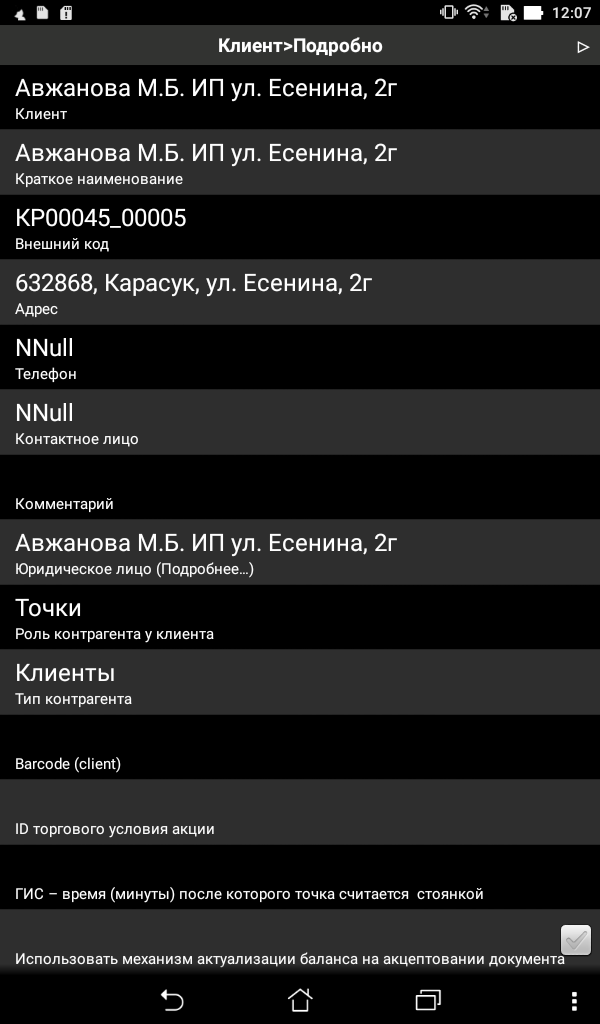
\includegraphics[width=0.8\linewidth]{scr14_1.png}}
		\ffigbox{\caption{Выделение клиентов с просроченными задолженностями}\label{pic:pic14_2}}%
		{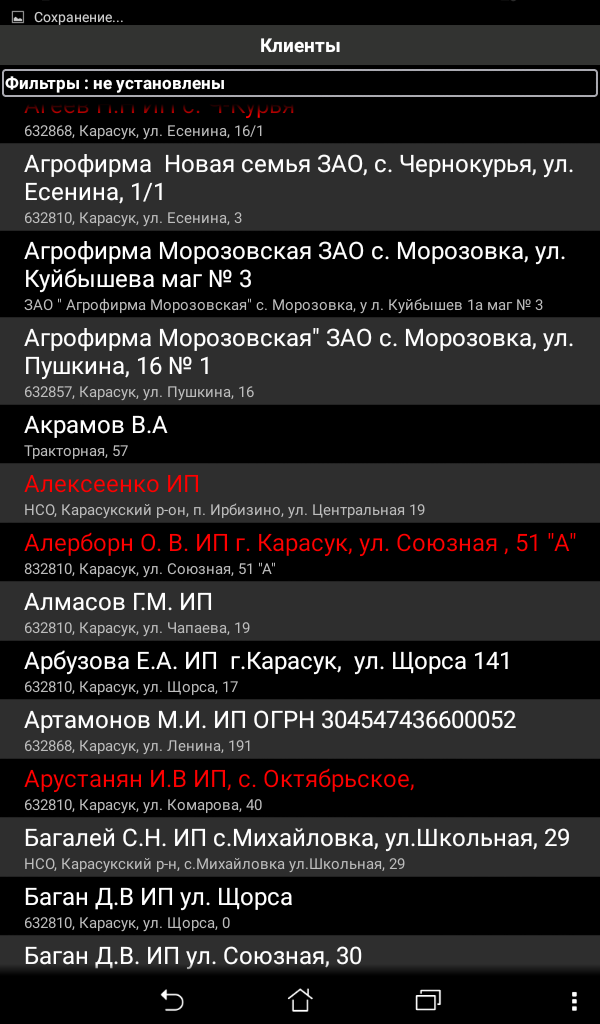
\includegraphics[width=0.8\linewidth]{scr14_2.png}}         
	\end{floatrow}
\end{figure}
\item Выделение клиентов с просроченными задолженностями
В Системе предусмотрено выделение записи о клиенте красным цветом в случае, если у клиента имеется просроченная задолженность.(рис.\ref{pic:pic14_2})
\end{enumerate}%Описание раздела <<Клиенты>>
\section{Описание раздела <<Товары>>}\label{sec:sec14_1}
\begin{enumerate}[\thesection .1]
\item Модуль служит для просмотра информации об остатках товара на центральных складах предприятия (рис.\ref {pic:pic15_1}). Также поддерживаются следующие функции: 
\begin{itemize}
	\item Просмотр списка товаров (с возможностью просмотра остатков товаров на вэн-складе \footnote{Вэн-склад - мобильный склад торгового представителя (кузов).} и на центральном складе);
	\item Просмотр детальной информации по товару;
	\item Установка единиц измерения товаров;
	\item Просмотр цен товаров (прайс-листов);
\end{itemize}
\item В каждом элементе списка содержатся:
\begin{itemize}
	\item Краткое наименование товара;
	\item Остаток товара на вэн-складе;
	\item Остаток товара на центральном складе;
	\item Наименование единицы измерения.
\end{itemize}

\begin{figure}[!h]
	\begin{floatrow}
		\ffigbox{\caption{Окно Товары}\label{pic:pic15_1}}%
		{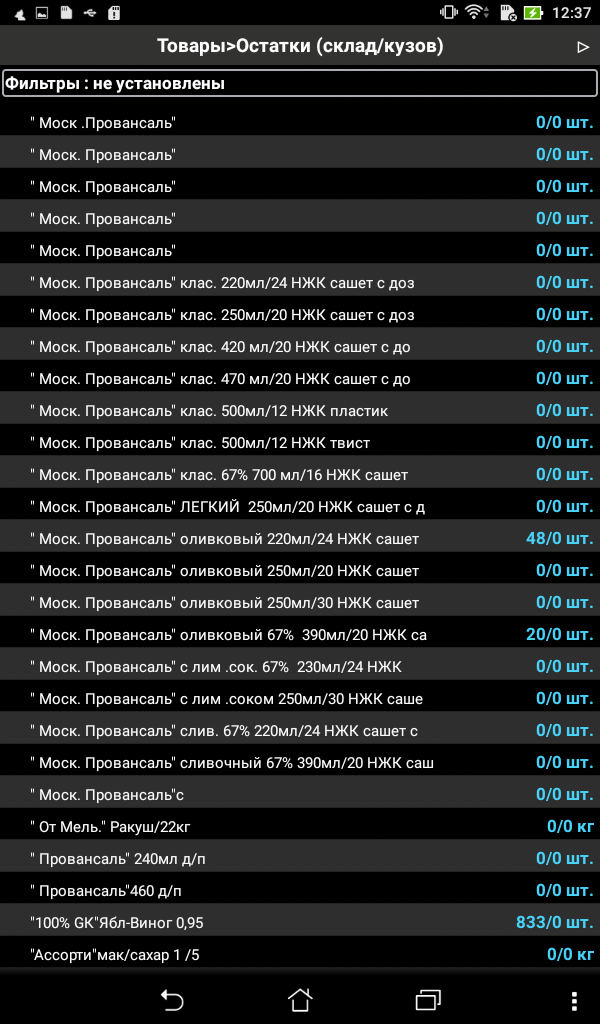
\includegraphics[width=0.8\linewidth]{scr15_1.png}}
		\ffigbox{\caption{Цены}\label{pic:pic15_2}}%
		{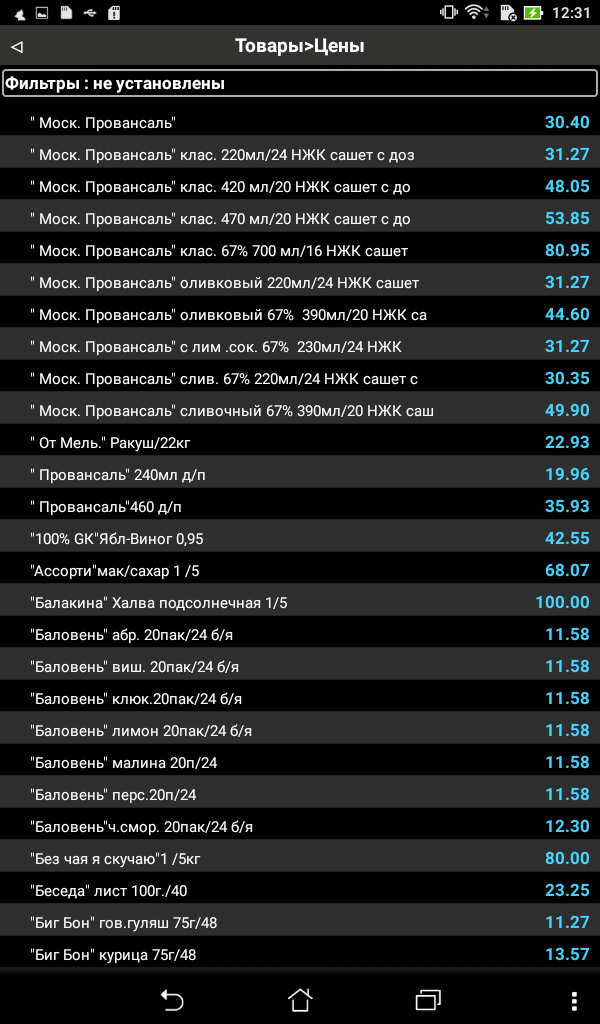
\includegraphics[width=0.8\linewidth]{scr15_2.png}}         
	\end{floatrow}
\end{figure}
\item Фильтры, доступные в окне: \footnote{Чтобы осуществить переход в окно выбора фильтров нужно произвести длительное касание в области фильтров. При коротком касании в области фильтров производится переход к окну выбора узла в иерархическом списке (фильтр «Каталог»).}
\begin{itemize}
	\item Каталог (фильтр по узлу номенклатурой иерархии);
	\item Количество (>0 или любое);
	\item Склад;
	\item MML;
	\item Атрибут;
	\item Значение;	
\end{itemize}
\item При скользящем касании справа - налево открывается окно просмотра цен (рис.\ref {pic:pic15_2}). 
В каждом элементе списка представлен товар и цена на него по прайс-листу, установленному в области фильтров.
Фильтры, доступные в окне просмотра цен товаров:
\begin{itemize}
	\item Каталог (фильтр по узлу номенклатурой иерархии);
	\item Прайс-лист (обязательный изменяемый фильтр);
	\item Склад;
	\item MML;
	\item Атрибут;
	\item Значение;	
\end{itemize}
\item Окно детальной информации о товаре
Для того чтобы перейти в окно просмотра детальной информации о товаре
\textbf{(Товары > Подробно)}  выберите товар кратким касанием в окне просмотра остатков товаров \textbf{(Товары > Остатки)}. При выборе товара в окне просмотра цен товаров \textbf{(Товары > Цены)} также происходит переход в окно \textbf{(Товары > Подробно)}
(рис.\ref {pic:pic15_3}).
\begin{figure}[!h]
	\begin{floatrow}
		\ffigbox{\caption{Окно просмотра детальной информации по товару}\label{pic:pic15_3}}%
		{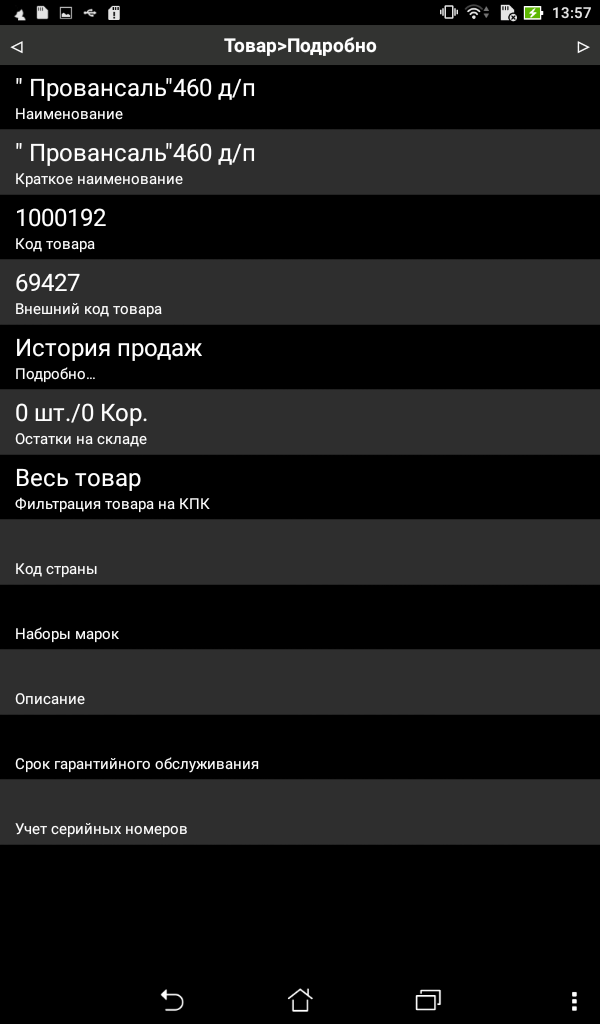
\includegraphics[width=0.8\linewidth]{scr15_3.png}}
		\ffigbox{\caption{Окно просмотра единиц измерения
				}\label{pic:pic15_4}}%
		{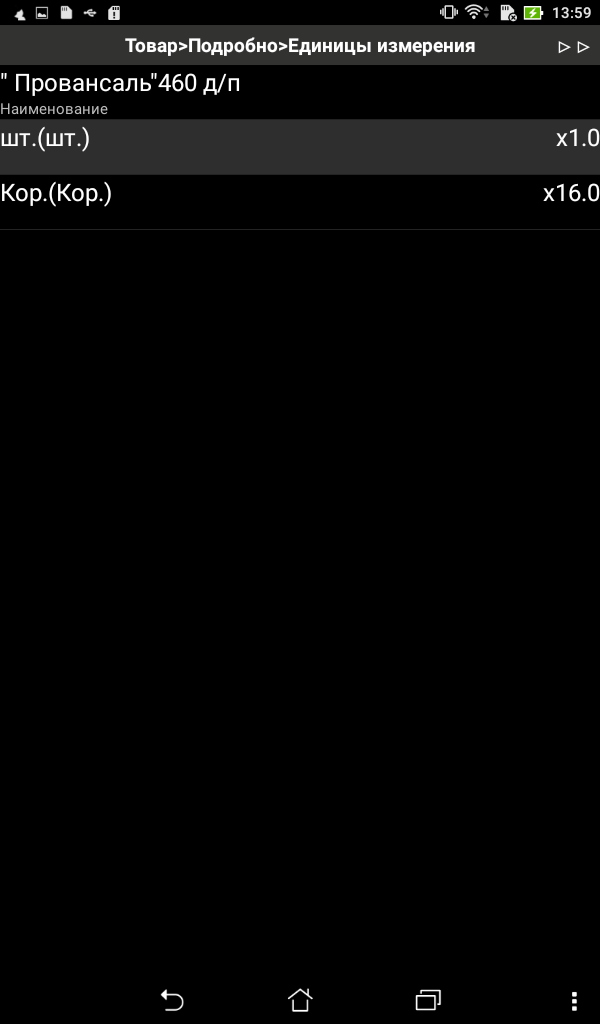
\includegraphics[width=0.8\linewidth]{scr15_4.png}}         
	\end{floatrow}
\end{figure}
В окне \textbf{(Товары > Подробно)} отображаются: 
\begin{itemize}
	\item Полное и краткое наименование товара;
	\item Код товара;
	\item Остатки на складе;
	\item Дополнительные атрибуты товара, сконфигурированные в конкретной системе.
\end{itemize}
\item При скользящем касании экрана слева - направо происходит переход в окно просмотра единиц измерения товара.(рис.\ref {pic:pic15_4}). 
В окне просмотра единиц измерения отображаются: 
\begin{itemize}
	\item Полное наименование товара;
	\item Cписок единиц измерений, присвоенных этому товару.
\end{itemize}
В каждом элементе списка содержится следующая информация:
\begin{itemize}
	\item Полное и краткое название ЕИ;
	\item Кратность ЕИ;
\end{itemize}
\end{enumerate}%Описание раздела <<Товары>>
\section{Описание раздела <<Баланс>>}
\begin{enumerate}[\thesection .1]
\item Модуль служит для просмотра списка клиентов и информации по их балансу (рис.\ref {pic:pic16_1}). В основном окне модуля отображается список клиентов, ограниченный параметрами установленных фильтров, и информация по балансу по каждому клиенту на соответствующую дату. 
\begin{figure}[!h]
	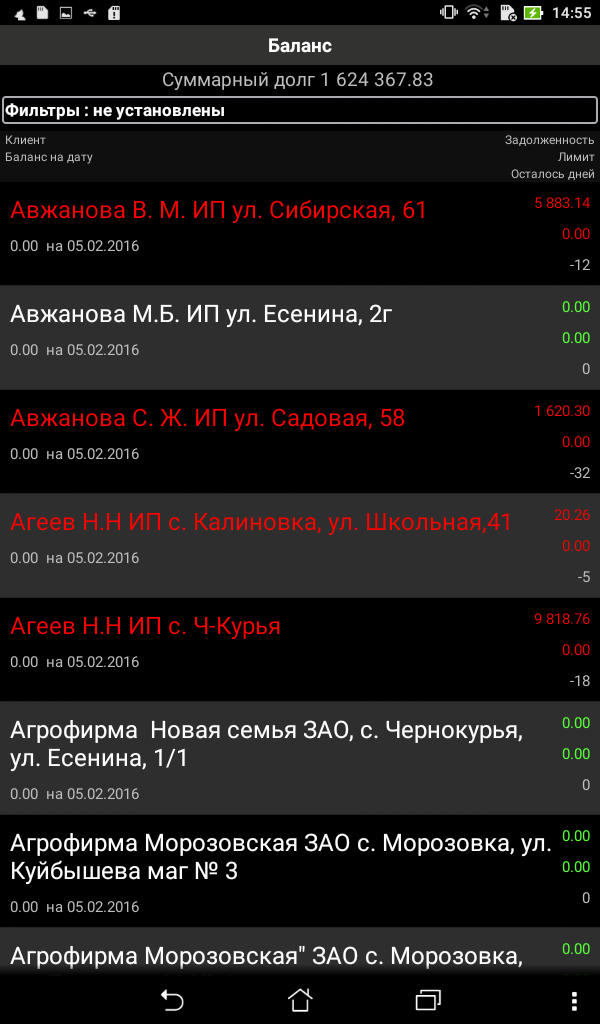
\includegraphics[width=0.4\linewidth]{scr16_1.png} 
	\caption{Баланс}\label{pic:pic16_1}
\end{figure}
Элемент списка содержит:
\begin{itemize}
	\item Наименование клиента;\footnote{Информация, отображаемая в данном поле, зависит от настроек Системы. В Системе возможно выводить в данное поле: наименование ТТ, наименование Хозяина ТТ или юр. лицо}
	\item Баланс на определённую дату;
	\item Справа от наименования клиента отображается размер задолженности клиента (в верхней строке);
	\item Кредитный лимит (в нижней строке).
\end{itemize}
Доступные фильтры:
\begin{itemize}
	\item Статус задолженности (все, без задолженности, с задолженностью и с просроченной задолженностью);
	\item Кредитное условие;
	\item Атрибут клиента;
	\item Значение атрибута клиента.
\end{itemize}
В случае если у того или иного клиента имеется просроченная задолженность,запись о таком клиенте может выделяться красным цветом. (в зависимости от настроек системы). 
%
\item Задолженность по документам
При нажатии на элемент списка в окне «Баланс» открывается окно  \textbf{(«Баланс > Подробно > Задолженности»)}. (рис.\ref {pic:pic16_2}) В данном окне отображается задолженность по оплате документов (Накладных, Накладных КИС), оформленных на выбранного клиента. 
\begin{figure}[!h]
	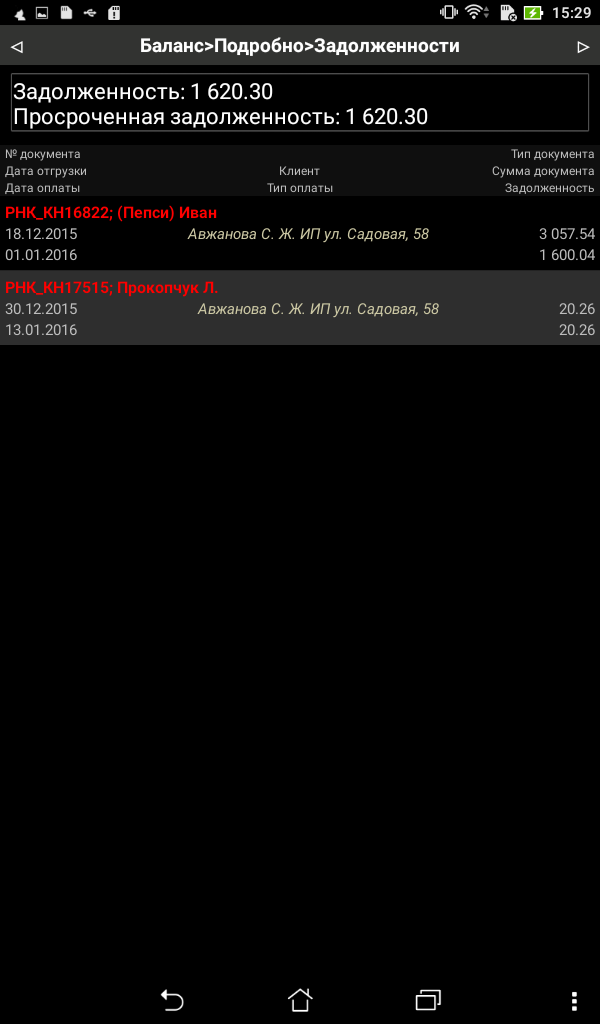
\includegraphics[width=0.3\linewidth]{scr16_2.png} 
	\caption{Задолжности}\label{pic:pic16_2}
\end{figure}
По каждому элементу списка отображается следующая информация:\footnote{Если дата оплаты документа-задолженности равна текущей дате, то номера таких документов выделяются в списке желтым цветом. Если дата оплаты документа меньше текущей даты, то номера таких документов выделяются в списке красным цветом. Остальные номера документов выделяются белым цветом.} 
\begin{itemize}
	\item № документа;
	\item Дата отгрузки – дата, на которую планируется отгрузка продукции по документу;
	\item Дата оплаты – дата, до которой клиент должен внести оплату;
	\item Клиент - наименование клиента, для которого зафиксирована задолженность;
	\item Тип оплаты – тип оплаты документа;
	\item Тип документа - тип документа, по которому зафиксирована задолженность;	
	\item Сумма документа – сумма, на которую был отгружен товар;
	\item Задолженность - сумма задолженности;	
\end{itemize}
\item История изменения баланса
Для просмотра истории изменения баланса выполните следующие действия: 
\begin{itemize}
	\item Нажмите на элемент списка в окне «Баланс»;
	\item В открывшемся окне \textbf{«Баланс > Подробно > Задолженности»} выполните скользящее касание справа – налево. Откроется окно \textbf{«Баланс > Подробно > Документы»};
\end{itemize}
В данном окне отображается история изменения задолженности выбранного клиента. Выводится список документов, повлиявших на текущую задолженность. По каждому элементу списка отображается следующая информация: 
\begin{itemize}
	\item № документа;
	\item Дата документа;
	\item Сумма - сумма по документу;
	\item Тип документа - краткое наименование типа документа;
	\item Баланс;	
\end{itemize}
%\item Баланс юридического лица
%Для просмотра информации о балансе юридического лица клиента выполните следующие действия: 
%\begin{itemize}
%	\item Нажмите на элемент списка в окне «Баланс»;
%	\item В открывшемся окне \textbf{«Баланс > Подробно > Задолженности»} выполните скользящее касание слева – направо. Откроется окно \textbf{«Баланс > Подробно > Юр. лица»}; 
%\end{itemize}
%В окне доступен фильтр по кредитному условию. По каждому элементу списка отображается следующая информация: 
%\begin{itemize}
%	\item Дата документа;
%	\item Баланс;
%	\item Задолженность – сумма задолженности;
%	\item Лимит;	
%\end{itemize}
\end{enumerate}%Описание раздела <<Баланс>>
\section{Описание раздела <<Настройки>>}
\begin{enumerate}[\thesection .1]
\item Модуль служит для настройки параметров Системы.(рис.\ref {pic:pic17_1},\ref {pic:pic17_2}).\\
\begin{figure}[h!]
	\begin{floatrow}
		\ffigbox{\caption{Модуль настройки 1}\label{pic:pic17_1}}%
		{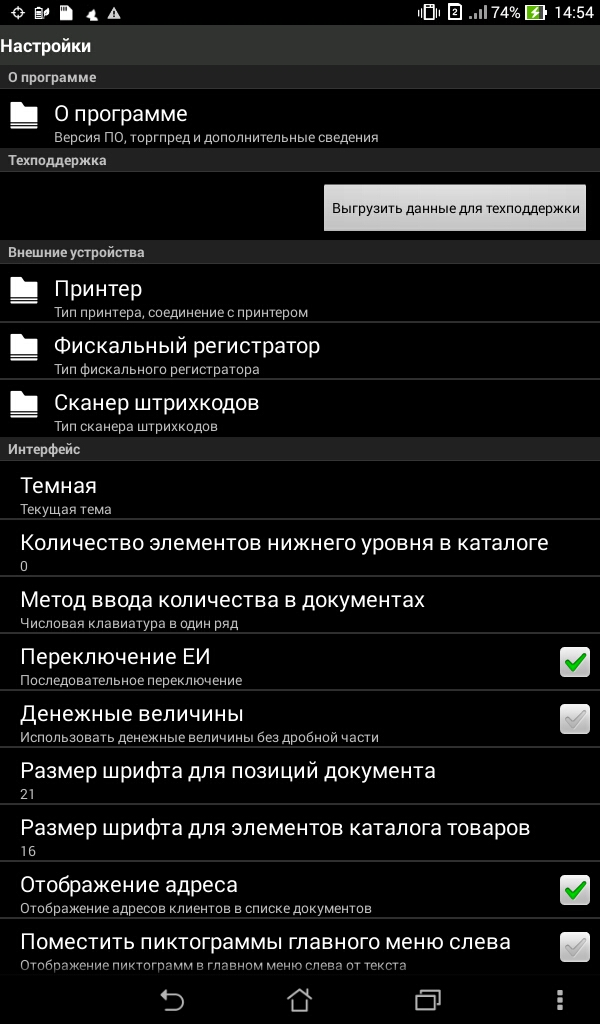
\includegraphics[width=0.6\linewidth]{scr17_1.jpg}}
		\ffigbox{\caption{Модуль настройки 2}\label{pic:pic17_2}}%
		{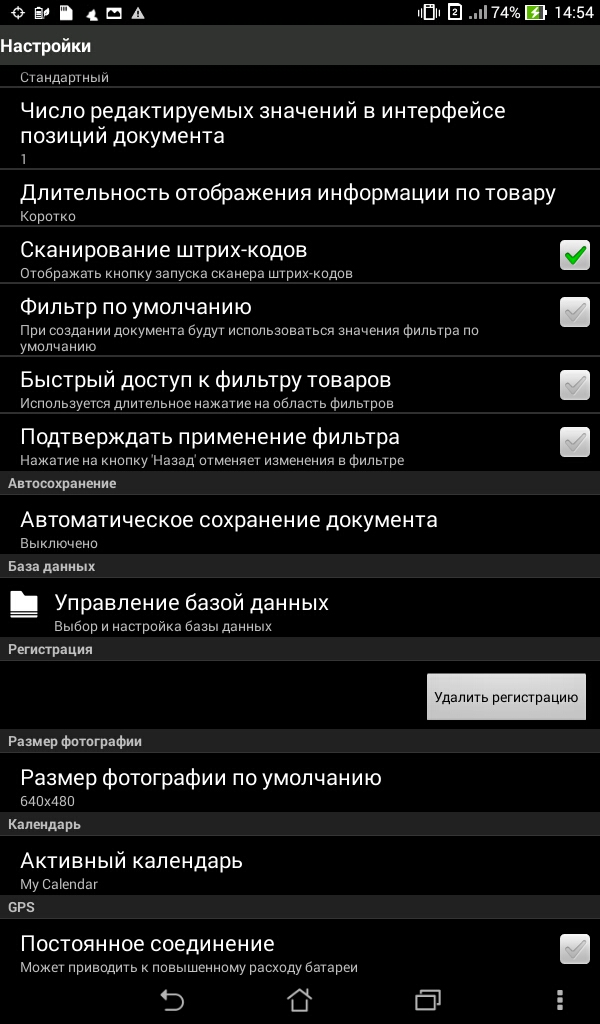
\includegraphics[width=0.6\linewidth]{scr17_2.jpg}}         
	\end{floatrow}
\end{figure}

\begin{longtable}{|p{5cm}|p{13cm}|}
\caption{Окно модуля содержит разделы, описанные в таблице ниже}\\
\hline	
\textbf{Название группы элементов} & \textbf{Описание группы элементов}\\ \hline
\endfirsthead
\hline
Название группы элементов & Описание группы элементов \\ \hline
\endhead
\hline
\multicolumn{2}{r}{Продолжение следует\ldots}\
\endfoot
\hline
\endlastfoot
%Название группы элементов & Описание группы элементов \\ \hline
О программе   & При касании на данном элементе открывается окно, где представлены следующие информационные поля: 
\begin{itemize}
	\item «Правовая информация»;
	\item «Версия Оптимум»;
	\item «Зарегистрировано» – содержит ФИО сотрудника, на которого произведена регистрация данного мобильного устройства в БД «Оптимум»;
\end{itemize} \\ \hline
Техподдержка  & Содержит кнопку, при нажатии на которую производится копирование служебных данных (логов, БД и настроек приложения) на SD-карту. Данные копируются в заархивированном виде.  \\ \hline
Внешние устройства  & Содержит поле «Принтер», по нажатию на которое открывается окно, в котором доступны следующие элементы:
 \begin{itemize}
 	\item «Тип принтера» - при касании на данном поле открывается окно выбора типа принтера (производителя);
 	\item «Тип соединения» - информационное поле, отображающее тип соединения с принтером;
 	\item «Имя (MAC-адрес) принтера» - при касании на данном поле открывается окно выбора принтера. В списке отображаются поддерживаемые Системой принтеры;
 \end{itemize} \\ \hline
Интерфейс  & Содержит поля:
\begin{itemize}
	\item «Количество элементов нижнего уровня в каталоге» - при касании на данном поле открывается окно для ввода значения данного параметра (N). Значение параметра определяет вид элемента иерархического списка - в каждом элементе списка будут показаны первые N значений из лежащего ниже уровня;
	\item «Вид клавиатуры» – параметр, который определяет, каким образом будет выглядеть клавиатура для ввода числовых значений (например, в окне ввода количества товарных позиций в документе). Возможны два режима: «Числовая клавиатура в один ряд» - цифры расположены в один ряд, «Увеличенная числовая клавиатура» - цифры расположены в два ряда;
	\item «Переключение ЕИ» - влияет на способ переключения единиц измерения товаров в документах. Возможны два режима:
	\begin{itemize}
		\item режим «Последовательное переключение»: при нажатии на кнопку единицы измерения (справа от поля ввода количества) происходит смена ЕИ для товарной позиции с ЕИ первого уровня на ЕИ второго уровня. Последующее нажатие приводит к смене ЕИ второго уровня на ЕИ третьего уровня и т. д;
		\item режим выбора: при нажатии на кнопку единицы измерения (справа от поля ввода количества) происходит открытие окна, где из списка выбирается необходимая ЕИ;
	\end{itemize}	
	\item «Денежные величины» (Использовать денежные величины без дробной части) - при активации данного режима все денежные величины (цены, суммы по документу) в приложении отображаются без дробной части. Дробная часть отсекается без округления;
	\item «Размер шрифта для позиций документа» - используется для установки размера шрифта при отображении информации о товарных позициях документа;
	\item «Размер шрифта для элементов каталога товаров» - используется для установки размера шрифта при отображении каталога товаров;
	\item «Отображение адреса» (Отображение адресов клиентов в списке документов) - при активации данного режима в списке созданных документов наряду с названием клиента отображается его адрес;
	\item «Компактный вид меню» (Использовать компактные строки в меню) - данный режим предназначен для отображения меню в более компактном виде (актуально, к примеру, для мобильных устройств с небольшим экраном);
\end{itemize}  \\ \hline
База данных  & Служебный функционал. Содержит поле «Управление базой данных», по нажатию на которое открывается окно просмотра доступных баз данных; \\ \hline
Регистрация  & Содержит кнопку «Удалить регистрацию», при нажатии на которую Система удаляет текущую регистрацию, после чего для работы с Системой необходима повторная регистрация и синхронизация устройства с сервером; \\ \hline
Размер фотографии  & Содержит поле «Размер фотографии по умолчанию», по нажатию на которое открывается окно выбора размера фотографий. Доступные размеры фотографий зависят от возможностей мобильного устройства; \\ \hline
Календарь  & Содержит поле «Активный календарь», по нажатию на которое открывается окно выбора календаря для отображения событий (задач), формируемых в модуле События;  \\ \hline
GPS  & Содержит поле «Приёмник GPS-координат», по нажатию на которое открывается окно выбора типа приёмника GPS-координат: \textbf{Location} или \textbf{NMEA}  \\ \hline
\end{longtable} 
\end{enumerate}%Описание раздела <<Настройки>>
\section{<<Принципы управления>>}
\begin{enumerate}[\thesection .1]
	\item Управление осуществляется путем касаний сенсорного экрана мобильного устройства(планшетного ПК). В качестве рабочего режима используется режим портретной ориентации.\\
	В процессе работы применяются следующие способы управления: \footnote{Функция "Мультитач" модулем "Оптимум" не поддерживается.}
	\begin{itemize}
		
		\item Касание экрана (аналог щелчка мышью в Windows);
		\item Долгое касание экрана или удержание (аналог двойного щелчка мышью в Windows); 
		\item Прокручивание (скользящее касание экрана); 
		\item Нажатие аппаратных кнопок («Назад», «Меню», «Поиск», «Домой»);
	\end{itemize}
\end{enumerate}%Описание раздела <<Принципы управления>>
\cleardoublepage
\addcontentsline{toc}{section}{\listfigurename}
%\pagestyle{empty}
%\listoffigures
%\cleardoublepage
\begingroup
\renewcommand\numberline[1]{}
%\listoffigures\thispagestyle{empty} \newpage
\emptypage\listoffigures\thispagestyle{empty} \newpage
\endgroup
%\listoffigures\thispagestyle{empty} \newpage
\end{document}

%enumerate latex \subsection
%
%If you need it only for a few enumerate environments, instead of setting globally
%
%\setlist[enumerate]{leftmargin=*,align=left,label=\thesubsection.\arabic*.}
%
%use these settings locally by issuing
%
%\begin{enumerate}[leftmargin=*,align=left,label=\thesubsection.\arabic*.]
%	
%	Note that you may need to load enumitem with the shortlabels option
%	
%	\usepackage[shortlabels]{enumitem}
%	
%	if you have already customized enumerate lists.


%http://tex.stackexchange.com/questions/227005/alignment-of-enumerate-numbered-by-subsection-and-the-existing-text

%http://tex.stackexchange.com/questions/1126/include-section-number-in-list-number

%latex list enumerate \subsection number

%\begin{wrapfigure}{l}{0.4\linewidth}
%\includegraphics[width=0.8\linewidth]{img/scr4.jpg} 
%\caption{Меню синхронизация}\label{pic:pic4}
%\end{wrapfigure}

%
%Соглашусь с тов. Const, что при хитром размещении картинок на титульном листе, может оказаться проще использовать точное позиционирование, например, посредством tikz: что-то вроде
%
%\begin{tikzpicture}
%\node at (0,0){\includegraphics{картинка}};
%\node at (1,0){\includegraphics{картинка}};
%\end{tikzpicture}